\documentclass[12pt,a4paper]{report}

% Compile with XeLaTeX or LuaLaTeX for Vietnamese text.
\usepackage{fontspec}
\usepackage{polyglossia}
\setmainlanguage{vietnamese}
\setmainfont{Times New Roman}

\usepackage[a4paper,left=3.5cm,right=2cm,top=2.5cm,bottom=2.5cm]{geometry}
\usepackage{graphicx}
\usepackage{booktabs}
\usepackage{array}
\usepackage{xcolor}
\usepackage{listings}
\usepackage{fancyvrb}
\usepackage{amsmath}
\usepackage{float}
\usepackage{caption}
\usepackage{chngcntr}
\usepackage{tikz}
\usetikzlibrary{arrows.meta, positioning}
\counterwithout{figure}{chapter}
\counterwithout{table}{chapter}
\usepackage[hidelinks]{hyperref}
\usepackage{caption}
\captionsetup[figure]{
    name=Hình,
    labelsep=colon,
    font=it
}
\captionsetup[table]{
    name=Bảng,
    labelsep=colon,
    font=it
}
\DeclareCaptionType{listing}[Đoạn mã]
\counterwithout{listing}{chapter}
\captionsetup[listing]{
    labelsep=colon,
    font=it,
    skip=2pt
}
\lstdefinestyle{pythoncode}{
    language=Python,
    basicstyle=\ttfamily\small,
    keywordstyle=\color{green!50!black}\bfseries,
    stringstyle=\color{orange!80!black},
    commentstyle=\color{teal!70!black}\itshape,
    emph={clean_text,text,re,BeautifulSoup},
    emphstyle=\color{blue!70!black}\bfseries,
    backgroundcolor=\color{gray!5},
    frame=single,
    rulecolor=\color{gray!20},
    numbers=left,
    numberstyle=\tiny\color{gray!60},
    stepnumber=1,
    numbersep=8pt,
    breaklines=true,
    columns=fullflexible,
    keepspaces=true,
    showstringspaces=false
}

\renewcommand{\contentsname}{MỤC LỤC}
\renewcommand{\listfigurename}{DANH MỤC HÌNH ẢNH}
\renewcommand{\listtablename}{DANH MỤC BẢNG}
\renewcommand{\bibname}{TÀI LIỆU THAM KHẢO}

\begin{document}

\begin{titlepage}
    \centering
    {\large BỘ GIÁO DỤC VÀ ĐÀO TẠO\par}
    \vspace{0.3cm}
    {\large TRƯỜNG ĐẠI HỌC ...\par}
    \vspace{2cm}
    {\Large \textbf{BÁO CÁO ĐỒ ÁN}\par}
    \vspace{1.5cm}
    {\LARGE \textbf{XÂY DỰNG HỆ THỐNG}\\
    \vspace{0.3cm}
    \textbf{PHÁT HIỆN BÀI BÁO TIẾNG VIỆT DO AI TẠO RA}\par}
    \vfill
    \begin{flushleft}
        \textbf{Sinh viên:} Nguyễn Hồ Giang Long\\
        \textbf{MSSV:} 2351010115\\
        \textbf{Giảng viên hướng dẫn:} Hồ Hướng Thiên
    \end{flushleft}
    \vfill
    TP. Hồ Chí Minh, 2026
\end{titlepage}

\pagenumbering{roman}

\chapter*{LỜI CẢM ƠN}
Nội dung lời cảm ơn của sinh viên được trình bày tại đây.
\addcontentsline{toc}{chapter}{LỜI CẢM ƠN}

\chapter*{NHẬN XÉT CỦA GIẢNG VIÊN HƯỚNG DẪN}
\vspace{8cm}
\addcontentsline{toc}{chapter}{NHẬN XÉT CỦA GIẢNG VIÊN HƯỚNG DẪN}

\tableofcontents
\listoffigures
\listoftables

\chapter*{DANH MỤC TỪ VIẾT TẮT}
\begin{tabular}{>{\bfseries}p{3cm}p{10cm}}
    AI & Artificial Intelligence - Trí tuệ nhân tạo \\
    API & Application Programming Interface \\
    BERT & Bidirectional Encoder Representations from Transformers \\
    LLM & Large Language Model \\
    XAI & Explainable Artificial Intelligence
\end{tabular}
\addcontentsline{toc}{chapter}{DANH MỤC TỪ VIẾT TẮT}

\chapter*{MỞ ĐẦU}
\addcontentsline{toc}{chapter}{MỞ ĐẦU}
\textbf{Lý do chọn đề tài:} Trình bày sự phát triển của nội dung do AI tạo ra và nhu cầu phát hiện văn bản AI tiếng Việt.

\textbf{Mục tiêu:} Xây dựng mô hình phân loại văn bản Human/AI và tích hợp mô hình vào một hệ thống web có khả năng giải thích kết quả.

\textbf{Đối tượng và phạm vi:} Văn bản tiếng Việt, ưu tiên nội dung IT/news; hệ thống gồm pipeline dữ liệu, mô hình BamiBERT, API và giao diện web.

\textbf{Phương pháp:} Thu thập dữ liệu, tiền xử lý, fine-tuning, đánh giá thực nghiệm và triển khai ứng dụng.

\textbf{Bố cục báo cáo:} Báo cáo gồm 5 chương nội dung, từ giới thiệu đề tài, cơ sở lý thuyết và dữ liệu đến đánh giá mô hình, triển khai hệ thống và phương hướng phát triển.

\clearpage
\pagenumbering{arabic}

% !TeX root = main.tex

% !TEX root = main.tex
\chapter{GIỚI THIỆU ĐỀ TÀI}

\section{Lý do chọn đề tài}
Trong bối cảnh hiện nay, sự bùng nổ và phát triển một cách chóng mặt của các mô hình ngôn ngữ lớn (Large Language Models - LLM) như ChatGPT, Claude, Gemini,\dots đã và đang làm thay đổi trong việc tạo ra và tiếp cận thông tin. Các mô hình này
có khả năng tạo ra những bài báo, văn bản hay tin tức một cách nhanh chóng và cách diễn đạt ngày càng tự nhiên, mạch lạc hơn, tức là ngày càng giống như con người viết. Điều này vô tình dẫn đến việc phân biệt nội dung giữa con người hay AI tạo ra
ngày càng khó hơn. Điều này làm tăng nhu cầu phát triển và gia tăng các phương pháp, hệ thống có khả năng phát hiện nội dung do AI tạo ra.

\vspace{\baselineskip}
\noindent Tuy nhiên, hiện nay, có một số nhóm người lại lợi dụng các mô hình ngôn ngữ lớn đó để tạo ra các bài báo, tin tức nhằm phát tán thông tin sai lệch, gây hoang mang dư luận, và sử dụng các bài báo từ nguồn khác để tạo ra các bài báo mới bằng 
cách viết, diễn đạt lại nội dung, lấy chất xám của người khác để tạo ra các sản phẩm cho riêng mình với mục đích khác. Ngoài ra, phần lớn các nghiên cứu và công cụ phát hiện văn bản do AI tạo ra hiện nay chỉ tập trung nhiều vào tiếng Anh, trong khi đó, các 
bài báo tiếng Việt vẫn chưa được quan tâm đúng mức.  

\vspace{\baselineskip}
\noindent Để góp phần giải quyết các vấn đề trên, em đã lựa chọn đề tài \textbf{“Phát hiện văn bản do AI tạo ra và viết lại"}, tập trung vào các bài báo, tin tức tiếng Việt về lĩnh vực công nghệ thông tin (IT), các thiết bị công nghệ hiện đại, AI,\dots Lý do chọn lĩnh vực đây là vì
em nghĩ đây là một lĩnh vực có nhiều thông tin, kiến thức mới được cập nhật liên tục và phát triển rất nhanh, có sự thay đổi thuật ngữ, từ vựng và cách diễn đạt liên tục, tạo ra một thách thức nhất định đối với bài toán phát hiện các văn bản do AI tạo ra. Qua đó, góp phần hỗ trợ quá
trình đánh giá và kiểm chứng nguồn gốc thông tin trên môi trường số. 

\section{Mục tiêu nghiên cứu}
Mục tiêu chính của đề tài là xây dựng một hệ thống có khả năng phát hiện các bài báo, văn bản do AI tạo ra hay người viết dựa trên kiến trúc mô hình BamiBert, đồng thời cũng đánh giá khả năng nhận diện nội dung tạo ra hay là viết lại bằng AI.
Bên cạnh khả năng phân loại, hệ thống còn hỗ trợ khả năng xác định mức độ đóng góp từng từ dựa vào kết quả dự đoán bằng thuật toán diễn giải mô hình (Explainable AI) Integrated Gradients và khả năng diễn giải kết quả bằng ngôn ngữ tự nhiên thông qua
API của Gemini. Hệ thống được triển khai dưới dạng web app, một giao diện tương tác người dùng thân thiện được thiết kế để người dùng có thể tương tác với hệ thống một cách dễ dàng.

\section{Đối tượng nghiên cứu}
Đối tượng nghiên cứu bao gồm:

\vspace{\baselineskip}
\noindent \textbf{Các bài báo do con người viết và AI tạo ra, viết lại:} Các bài báo, tin tức chuyên về lĩnh vực công nghệ thông tin, AI, công nghệ hiện đại,\dots được thu thập từ các nguồn uy tín, rõ ràng.

\vspace{\baselineskip}
\noindent \textbf{Các phương pháp và mô hình học sâu cho bài toán phân loại văn bản:} Nghiên cứu các mô hình học sâu xử lý các đặc trưng ngôn ngữ và phương pháp học biểu diễn văn bản tiếng Việt nhằm phân biệt nội dung
con người hay AI tạo ra, viết lại.

\vspace{\baselineskip}
\noindent \textbf{Phương pháp diễn giải mô hình (Explainable AI):} Nghiên cứu các phương pháp nhằm diễn giải kết quả dự đoán của mô hình học sâu, giải thích được mức độ đóng góp từng từ cho kết quả dự đoán.

\vspace{\baselineskip}
\noindent \textbf{Sử dụng API của Gemini:} Nghiên cứu khả năng diễn giải kết quả dự đoán bằng ngôn ngữ tự nhiên với một số ràng buộc nhất định.

\vspace{\baselineskip}
\noindent \textbf{Triển khai hệ thống web app:} Xây dựng một hệ thống đơn giản, dễ sử dụng, dữ liệu được lưu trữ bằng SQLite, triển khai trên Docker.

\section{Bố cục đề tài}
Chương 1: Giới thiệu đề tài 

\vspace{\baselineskip}
\noindent Chương 2: Các công nghệ và cơ sở lý thuyết 

\vspace{\baselineskip}
\noindent Chương 3: Dữ liệu, phương pháp xây dựng hệ thống

\vspace{\baselineskip}
\noindent Chương 4: Thực nghiệm và đánh giá hệ thống

\vspace{\baselineskip}
\noindent Chương 5: Kết luận và phương hướng phát triển hệ thống trong tương lai
% !TEX root = main.tex
\chapter{CÁC CÔNG NGHỆ VÀ CƠ SỞ LÝ THUYẾT}

\section{Xử lý ngôn ngữ tự nhiên}
\subsection{Vai trò của xử lý ngôn ngữ tự nhiên}
Xử lý ngôn ngữ tự nhiên (Natural Language Processing - NLP) là một lĩnh vực của trí tuệ nhân tạo (Artificial Intelligence - AI) tập trung vào việc phân tích và xử lý các bài toán liên quan tới ngôn ngữ tự nhiên giúp cho máy tính có thể hiểu, phân tích và khai thác thông tin từ chính các bài toán đó.

\begin{figure}[H]
    \centering
    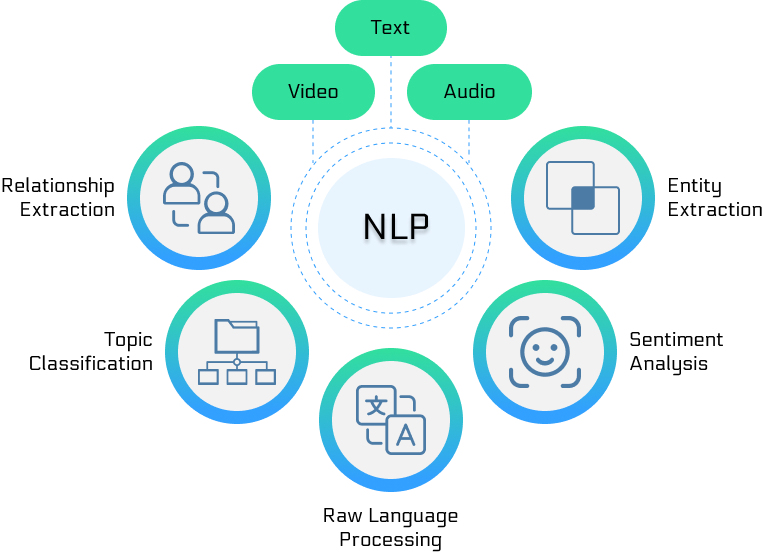
\includegraphics[width=0.8\textwidth]{images/chapter_02/img_01.png}
    \caption{Xử lý ngôn ngữ tự nhiên - Natural Language Processing}
    \label{fig:nlp}
\end{figure}

\noindent 
Khác với dữ liệu số hoặc dữ liệu có cấu trúc, dữ liệu văn bản ngôn ngữ tự nhiên có nhiều đặc điểm phức tạp, chẳn hạn như ngữ nghĩa, ngữ cảnh, cách sử dụng từ và cấu trúc câu. Do đó, NLP đóng vai trò quan trọng trong việc chuyển đổi văn bản thành dạng dữ liệu có thể đưa vào các mô hình học máy và học sâu xử lý.

\subsection{Biểu diễn văn bản và embedding}
Để cho máy tính có thể hiểu được văn bản, nội dung của văn bản đó sẽ được chuyển đổi sang dạng biểu diễn số. Một trong những phương pháp phổ biến để giải quyết được yêu cầu đó là chuyển đổi văn bản dưới dạng vector số, trong đó mỗi vector đều mang, chứa đựng các thông tin bao gồm: ý nghĩa, ngôn ngữ, cấu trúc của từ, cụm từ và câu. Các phương pháp truyền thống như Bag-of-Words hoặc TF-IDF chủ yếu biểu diễn vector dựa vào sự xuất hiện và tần suất của từ, vẫn chưa đủ khả năng
để phản ánh đầy đủ mối quan hệ ngữ nghĩa và ngữ cảnh của từ trong câu.

\vspace{\baselineskip}
\noindent
Embedding là một kĩ thuật chuyển đổi dữ liệu văn bản thô như từ ngữ, câu văn, hình ảnh hay là âm thanh sang một vector trong không gian đa chiều. Mỗi đơn vị mà có ý nghĩa tương đồng thì các vector của chúng sẽ được biểu diễn gần nhau trong không gian đa chiều đó. Nhờ vậy, embedding có thể giúp cho mô hình máy có thể hiểu và khai thác tốt hơn những đặc điểm ngữ nghĩa thay vì chỉ dựa trên sự xuất hiện riêng lẻ của từng từ.

\begin{figure}[H]
    \centering
    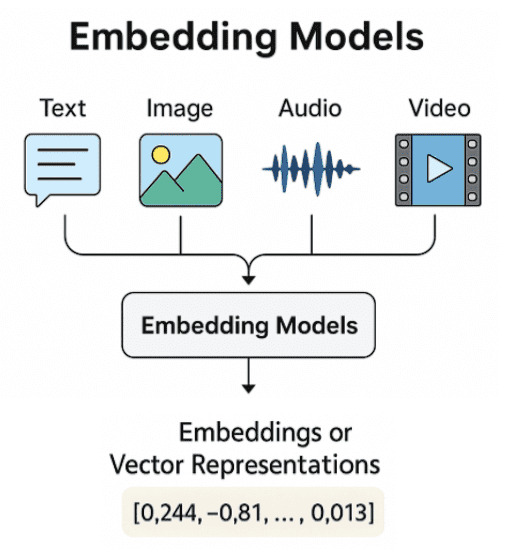
\includegraphics[width=0.4\textwidth]{images/chapter_02/img_02.jpg}
    \caption{Biểu diễn dữ liệu thô dưới dạng vector embedding}
    \label{fig:nlp}
\end{figure}

\noindent
Trong các hệ thống xử lý văn bản hiện tại, embedding là thành phần rất quan trọng trong việc hỗ trợ chuyển đổi dữ liệu dạng ngôn ngữ tự nhiên sang dữ liệu số, hay là vector để máy tính có thể hiểu, xử lý và tính toán được. Các vector embedding đó sẽ được đưa vào các mô hình học để thực hiện một số tác vụ như phân loại văn bản, tìm kiếm thông tin, phát hiện tương đồng và phân
tích ngữ nghĩa.

\vspace{\baselineskip}
\noindent
Đối với bài toán phân loại văn bản AI tạo ra, việc biểu diễn văn bản dưới dạng dữ liệu số có thể giúp cho các mô hình khai thác tốt đặc trưng từ dữ liệu đầu vào, tăng khả năng nhận diện được các văn bẳn do người viết hay do AI tạo ra. Tuy vậy, chất lượng biểu diễn các đặc trưng cũng góp phần cực kỳ quan trọng, ảnh hưởng trực tiếp đến kết quả đầu ra trong việc phân loại và đánh giá của mô hình.

\section{Mô hình Transformer và BERT}
\subsection{Kiến trúc Transformer}
Transformer là một kiến trúc mạng nơ-ron được thiết kế nhằm mục đích xử lý dữ liệu tuần tự, đặc biệt hiệu quả đối với các bài toán xử lý ngôn ngữ tự nhiên. Khác với các kiến trúc tuần tự như Recurrent Neural Network (RNN) và Long Short-Term Memory (LSTM), Transformer có khả năng xử lý các token trong chuỗi một cách đồng thời, không theo tuần tự. Có nghĩa là, mô hình sẽ tính toán mức độ liên quan của một token
so với các token khác tồn tại trong chuỗi. Nhờ đó, một token sẽ mang ý nghĩa phù hợp với ngữ cảnh, tức là phù hợp với ý nghĩa của câu đó mà không phải phụ thuộc vào mỗi bản thân của token đó.

\begin{figure}[H]
    \centering
    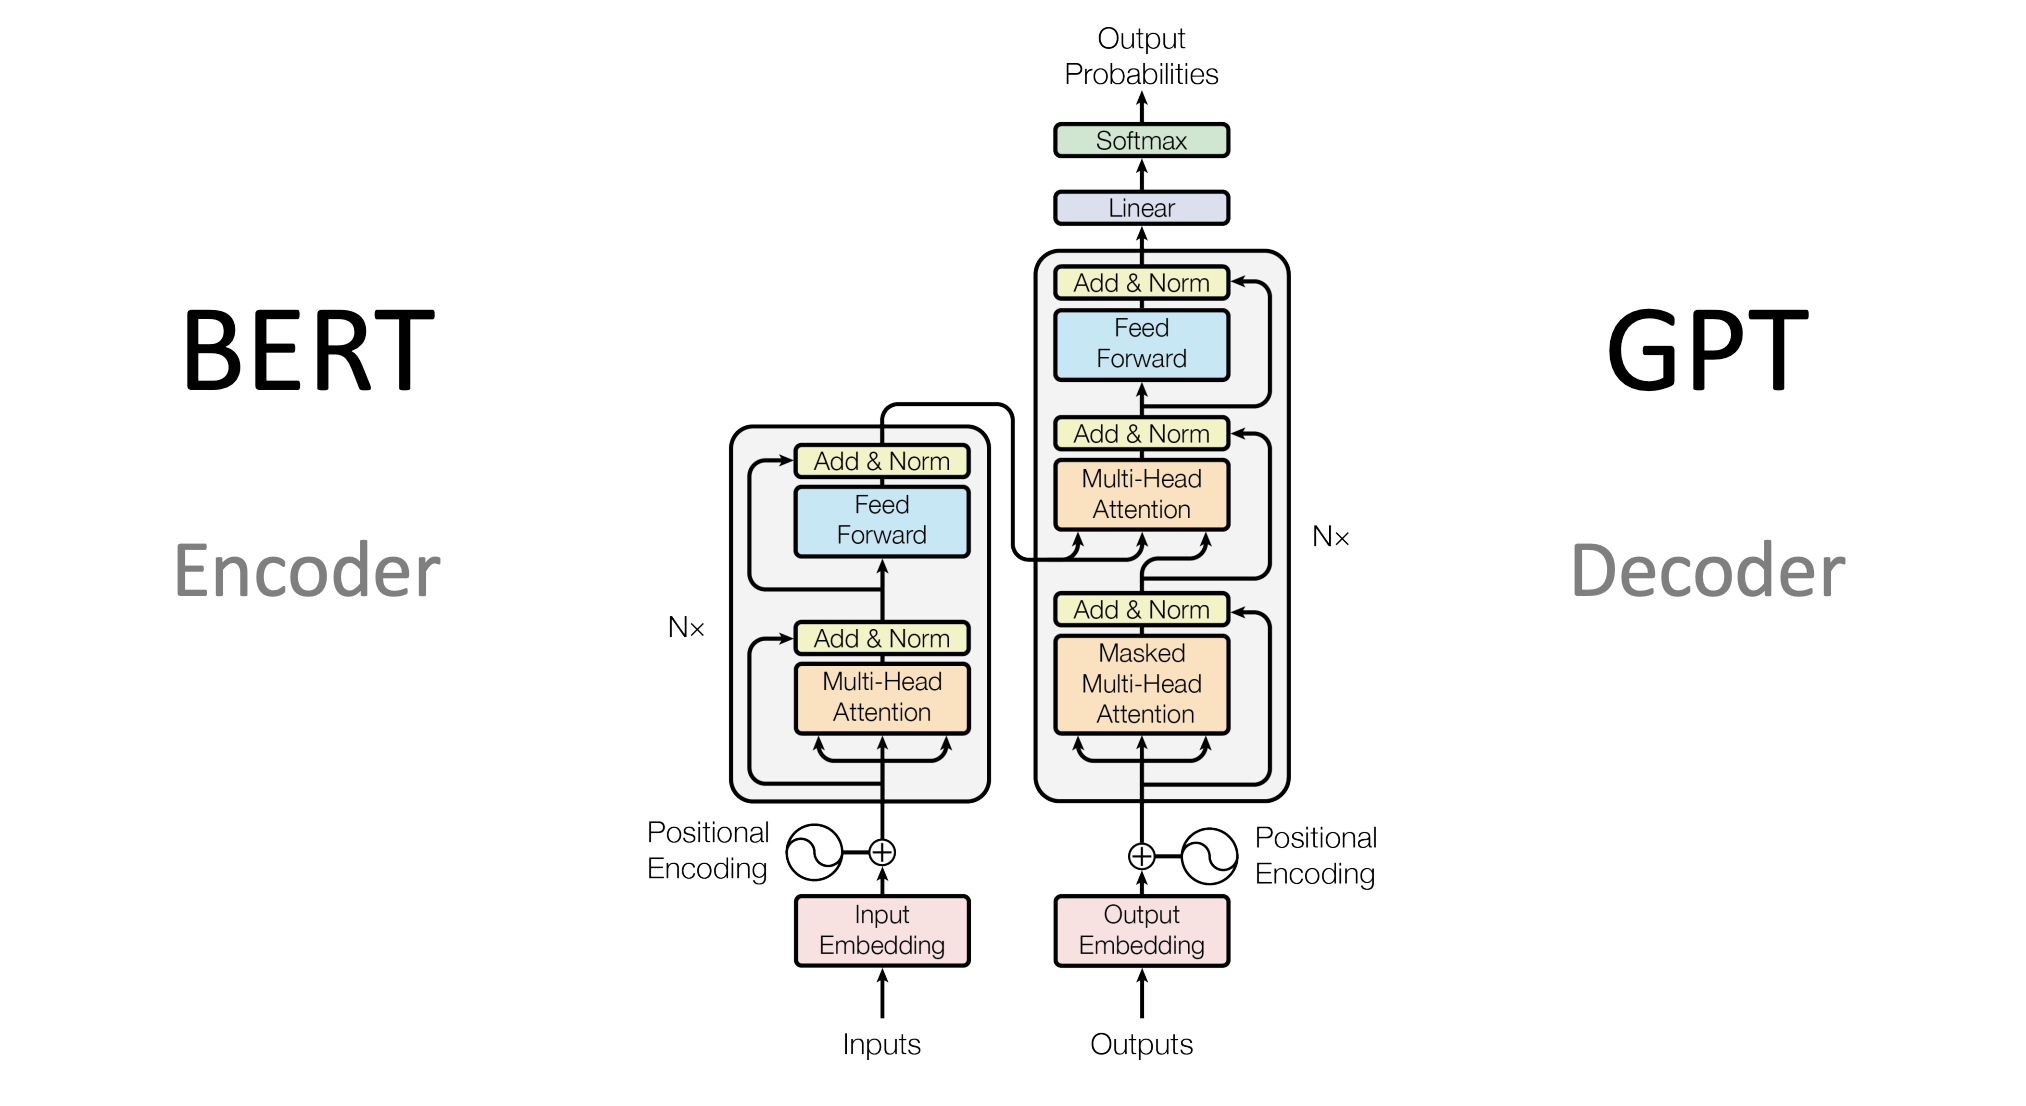
\includegraphics[width=1.0\textwidth]{images/chapter_02/img_03.png}
    \caption{Kiến trúc mô hình Transformer}
    \label{fig:nlp}
\end{figure}

\noindent
Cơ chế mà xác định mức độ quan trọng của từng token dựa vào các token lân cận có trong chuỗi được gọi là cơ chế tự chú ý (Self-Attention). Qua đó, Transformer có khả năng mô hình hóa các mối quan hệ phụ thuộc xa trong văn bản, tức là một token cần thêm thông tin từ một token rất xa trong văn bản, một đặc điểm quan trọng đối với các bài toán xử lý ngôn ngữ tự nhiên.

\vspace{\baselineskip}
\noindent
Transformer gồm tất cả là hai thành phần, Encoder và Decoder. Phần đầu là Encoder, dữ liệu đầu vào sẽ được chia thành các token (Tokenization) rồi sau đó sẽ embedding thành các vector. Tiếp theo, các vector đó sẽ được qua một lớp, gọi là Positional Embedding, lớp này sẽ có trách nhiệm embedding thành các vector có tính đại diện vị trí của từ trong chuỗi dữ liệu đó, ví dụ như: "I love AI" và "AI love I" thì mô hình nhìn có vẻ giống nhau nhưng thực tế
thì không phải vậy, thế nên là lớp Positional Embedding góp phần rất là quan trọng. Qua đó, ta sẽ có được một vector vừa có thông tin về ngữ nghĩa và vị trí của từ đó trong câu. Sau đó, các vector embedding sẽ được đưa vào lớp tự chú ý (Self-Attention) như đã nói ở trên, mỗi từ sẽ được ánh xạ thành ba thành phần: Query (Q) - từ này đang tìm kiếm cái gì, Key (K) - từ này yêu cầu cái gì, và Value (V) - thông tin thực sự mà từ này mang lại lại gì. Mỗi từ 
sẽ sử dụng Q để tính tích vô hướng so với các K của các từ còn lại, giá trị vừa tính được sẽ được chuẩn hóa thành các khoảng giá trị có thể xử lý được rồi sẽ đưa vào hàm Softmax để đưa thành các giá trị xác suất [0, 1].

\vspace{\baselineskip}
\noindent
Sau đó, dữ liệu sẽ đi qua lớp đa đầu tự chú ý (Multi-Head Self Attention), lớp này đảm bảo cho việc chú ý sẽ chạy song song, mỗi đầu tập trung vào một công việc riêng, ví dụ như một đầu tập trung vào mối quan hệ chủ ngữ - động từ, một đầu tập trung vào tính từ đó mô tả danh từ nào. Tiếp theo, dữ liệu sẽ được đưa vào lớp mạng nơ-ron truyển thằng (Feed-Forward Network), lớp này sẽ hỗ trợ cho việc đào sâu thông tin của từng từ hơn, ý nghĩa chính xác hơn và loại bỏ nhiễu kết hợp với các lớp
Add \& Norm để ổn định quá trình học hơn. Phần Decoder cũng có cấu trúc tương tự như Encoder nhưng thêm một lớp là Masked Multi-Head Attention, là lớp che đi các token phía sau của token đang xét để nó không biết trước thông tin. Điều này tránh rò rỉ thông tin trong quá trình học. Các khối Encoder và Decoder có thể lặp lại nhiều lần.

\subsection{BERT và BamiBERT}
BERT (Bidirectional Encoder Representations from Transformers) là một mô hình ngôn ngữ tiền huấn luyện được phát triển dựa trên kiến trúc Transformer Encoder. Nhờ vậy, mỗi token có thể khai thác thông tin từ hai chiều, phía trước và phía sau của token đang xét nên mô hình có khả năng nắm bắt tốt mối quan hệ các từ dựa trên ngữ cảnh của câu.

\vspace{\baselineskip}
\noindent
BERT được tiền huấn luyện trên một bộ lượng lớn văn bản thông qua nhiều nhiệm vụ học ngôn ngữ khác nhau, trong đó phổ biến nhất là mô hình ngôn ngữ che giấu (Masked Language Modeling - MLM). Cụ thể, trong nhiệm vụ này thì một số token trong câu sẽ bị che lại (masked) và mô hình có nhiệm vụ phải dự đoán các token bị che đó dựa vào các token còn lại. Quá trình này hỗ trợ cho mô hình BERT học được các đặc trưng của từ vựng, ngữ nghĩa và mối quan hệ giữa các thành phần trong văn bản.

\vspace{\baselineskip}
\noindent
Sau giai đoạn tiền huấn luyện, BERT có thể được fine-tune, tức là tinh chỉnh, huấn luyện trên tập dữ liệu của mình cho nhiều tác vụ khác nhau. Cụ thể trong bài toán phân loại văn bản, các biểu diễn thu được, tức là các vector embedding từ dữ liệu ban đầu từ BERT sẽ được đưa vào một lớp phân loại để dự đoán nhãn tương ứng. Cách tiếp cận này tận dụng kiến thức mà mô hình đã học được trong quá trình tiền huấn luyện thay vì xây dựng lại từ đầu

\vspace{\baselineskip}
\noindent
BamiBERT là một mô hình được xây dựng dựa trên kiến trúc BERT, được huấn luyện trên phần lớn các tập dữ liệu tiếng Việt với nhiều tác vụ khác nhau, bao gồm suy luận ngôn ngữ, nhận dạng thực thể, phân tích cảm xúc, phân loại chủ đề, phát hiện spam và phân tích khía cạnh.

\begin{figure}[H]
    \centering
    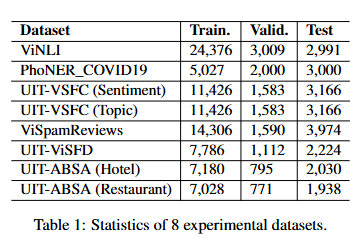
\includegraphics[width=0.6\textwidth]{images/chapter_02/img_04.png}
    \caption{Các tập dữ liệu dùng để huấn luyện BamiBERT}
    \label{fig:nlp}
\end{figure}

\noindent
Trong hệ thống, BamiBERT đóng vai trò là một mô hình biểu diễn các đặc trưng và sau đó biểu diễn này được sử dụng cho nhiệm vụ phân loại các lớp để đưa ra dự đoán. Việc sử dụng mô hình tiền huấn luyện giúp hệ thống tận dụng được các đặc trưng ngôn ngữ đã học trước đó và phù hợp hóa với bài toán phát hiện nội dung AI.

\begin{figure}[H]
    \centering
    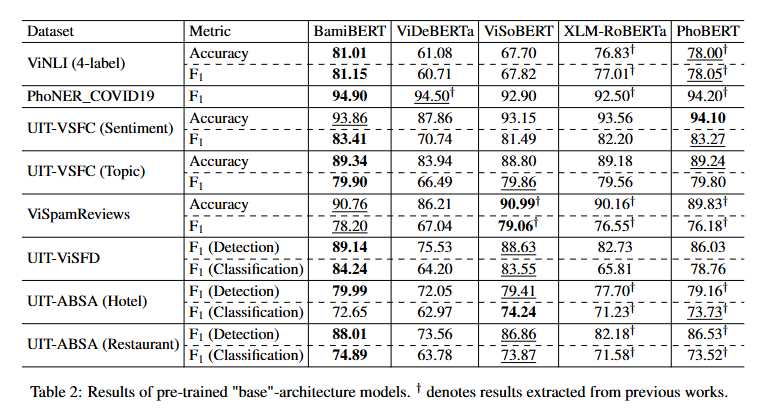
\includegraphics[width=1.0\textwidth]{images/chapter_02/img_05.png}
    \caption{Kết quả dự đoán của BamiBERT so với các mô hình BERT khác}
    \label{fig:nlp}
\end{figure}

\noindent
Lý do lựa chọn BamiBERT làm mô hình trích xuất, phân loại cho đồ án này là vì độ chính xác của mô hình tốt hơn hẳn so với các mô hình BERT trước dựa vào bảng kết quả (Hình 5). Tuy nhiên, có thể trong một số bài toán khác, hay cụ thể là bài toán phân loại văn bản AI này thì một số mô hình BERT khác có khả năng xử lý tốt và đưa
ra độ chính xác cao hơn. Do đó, bảng kết quả trên chỉ là thước đo cơ sở để lựa chọn mô hình BamiBERT nhưng về vấn đề xử lý hay độ chính xác cao hơn thì có thể các mô hình BERT khác tốt hơn so với BamiBERT.

\subsection{Token \texttt{[CLS]} và vector đại diện cho câu}
Trong kiến trúc BERT, token \texttt{[CLS]} (Classification) là một token đặc biệt được thêm vào vị trí đầu tiên của chuỗi đầu vào. Token này có nhiệm vụ tổng hợp toàn bộ thông tin của chuỗi đang xử lý thông qua các lớp Encoder của Transformer. Trong quá trình xử lý chuỗi, cơ chế Self-Attention sẽ cho phép token \texttt{[CLS]} tương tác với tất cả các token còn lại trong chuỗi, nhờ đó mà thu
được ngữ cảnh của toàn bộ văn bản trong chuỗi.

\begin{figure}[H]
    \centering
    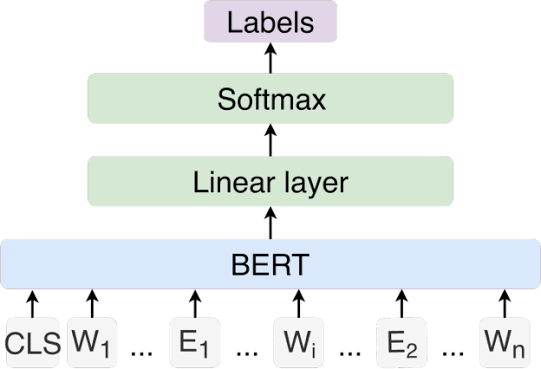
\includegraphics[width=0.6\textwidth]{images/chapter_02/img_06.png}
    \caption{Token \texttt{[CLS]} trong chuỗi}
    \label{fig:nlp}
\end{figure}

\noindent
Sau khi chuỗi đầu vào đi qua các lớp Encoder, mỗi token sẽ có một vector embedding tương ứng. Tuy nhiên, token \texttt{[CLS]} có một vector đặc biệt, là vector đại diện cho toàn bộ câu trong chuỗi. Vector này chứa toàn bộ thông tin ngữ cảnh của chuỗi đầu vào và được sử dụng cho các bài toán phân loại. Cụ thể, trong bài toán của đồ án này, vector biểu diễn của token \texttt{[CLS]} từ BamiBERT được sử dụng làm đầu vào cho Classification Head, sau đó vector này sẽ được
chuyển đổi thành các giá trị tương ứng cho hai lớp Human và AI cho bài toán, cụ thể các giá trị đó là giá trị logit.

\subsection{Classification head}
Classification head là một lớp của mô hình BERT, cho phép nhận đầu vào là vector đại diện của token \texttt{[CLS]} để thực hiện nhiệm vụ phân loại. Thành phần này là cầu nối giữa mô hình tiền huấn luyện và nhiệm vụ phân loại cụ thể.

\vspace{\baselineskip}
\noindent
Trong bài toán phân loại của đồ án, lớp classification head nhận đầu vào sẽ nhận vector đại diện của BamiBERT làm đầu vào. Sau đó, vector này sẽ được đưa qua một lớp gọi là lớp kết nối đầy đủ (Fully Connected Layer) để ánh xạ từ không gian nhiều chiều của BamiBERT sang không gian nhãn của bài toán phân loại của đồ án, tức là đồ án chỉ gồm có hai lớp, AI và Human nên không gian của bài toán này chỉ có
hai chiều và giá trị là logit. Tiếp theo, các giá trị này sẽ được trực tiếp đưa vào hàm Softmax để chuyển đổi thành các giá trị xác suất làm kết quả dự đoán.

\subsection{Fine-tune mô hình tiền huấn luyện}
Fine-tune là quá trình tiếp tục huấn luyện mô hình đã được tiền huấn luyện trên một tập dữ liệu cụ thể, một bài toán mà ta đang giải quyết. Tức là thay vì khởi tạo các tham số lại từ đầu thì quá trình này sẽ tận dụng các tham số mà mô hình này đã học được trong quá trình tiền huấn luyện, rồi điều chỉnh sao cho phù hợp với mục tiêu của bài toán.

\begin{figure}[H]
    \centering
    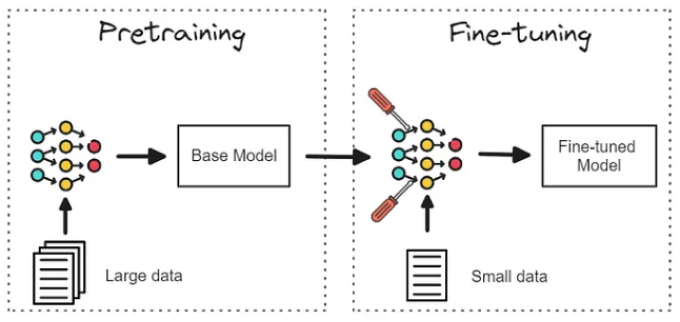
\includegraphics[width=0.8\textwidth]{images/chapter_02/img_07.jpg}
    \caption{Quá trình fine-tuning}
    \label{fig:nlp}
\end{figure}

\noindent
Đối với mô hình BamiBERT được sử dụng trong đồ án, giai đoạn tiền huấn luyện ban đầu đã phần lớn giúp cho mô hình đã học được các dữ liệu tiếng Việt. Tuy nhiên, mô hình này vẫn chưa được huấn luyện tối ưu cho bài toán phân loại, cụ thể là phân loại tin tức AI hay là Human. Do đó, đồ án thực
hiện fine-tune mô hình trên tập dữ liệu của bài toán, đồng thời kết hợp thêm lớp Classification Head để thực hiện phân loại văn bản đó là người hay AI tạo ra.


\section{Thuật toán diễn giải mô hình (Explainable AI - XAI)}
\subsection{Khái niệm Explainable AI}
Thuật toán diễn giải mô hình (Explainable AI) là một nhóm, tập hợp các phương pháp và kĩ thuật giúp cho con người cái cách mà một mô hình AI đưa ra dự đoán. Trong mô hình học sâu, thông thường thì quá trình dự đoán rất khó giải thích trực tiếp vì mô hình chứa rất nhiều tham số và thực hiện các thuật toán, quá trình 
tính toán cực kỳ phức tạp. XAI cung cấp phương pháp, thuật toán để giải thích mối quan hệ giữa dữ liệu đầu vào so với kết quả đầu ra của mô hình, điều này góp phần lớn cho việc giải thích minh bạch, dễ hiểu cho người dùng.

\begin{figure}[H]
    \centering
    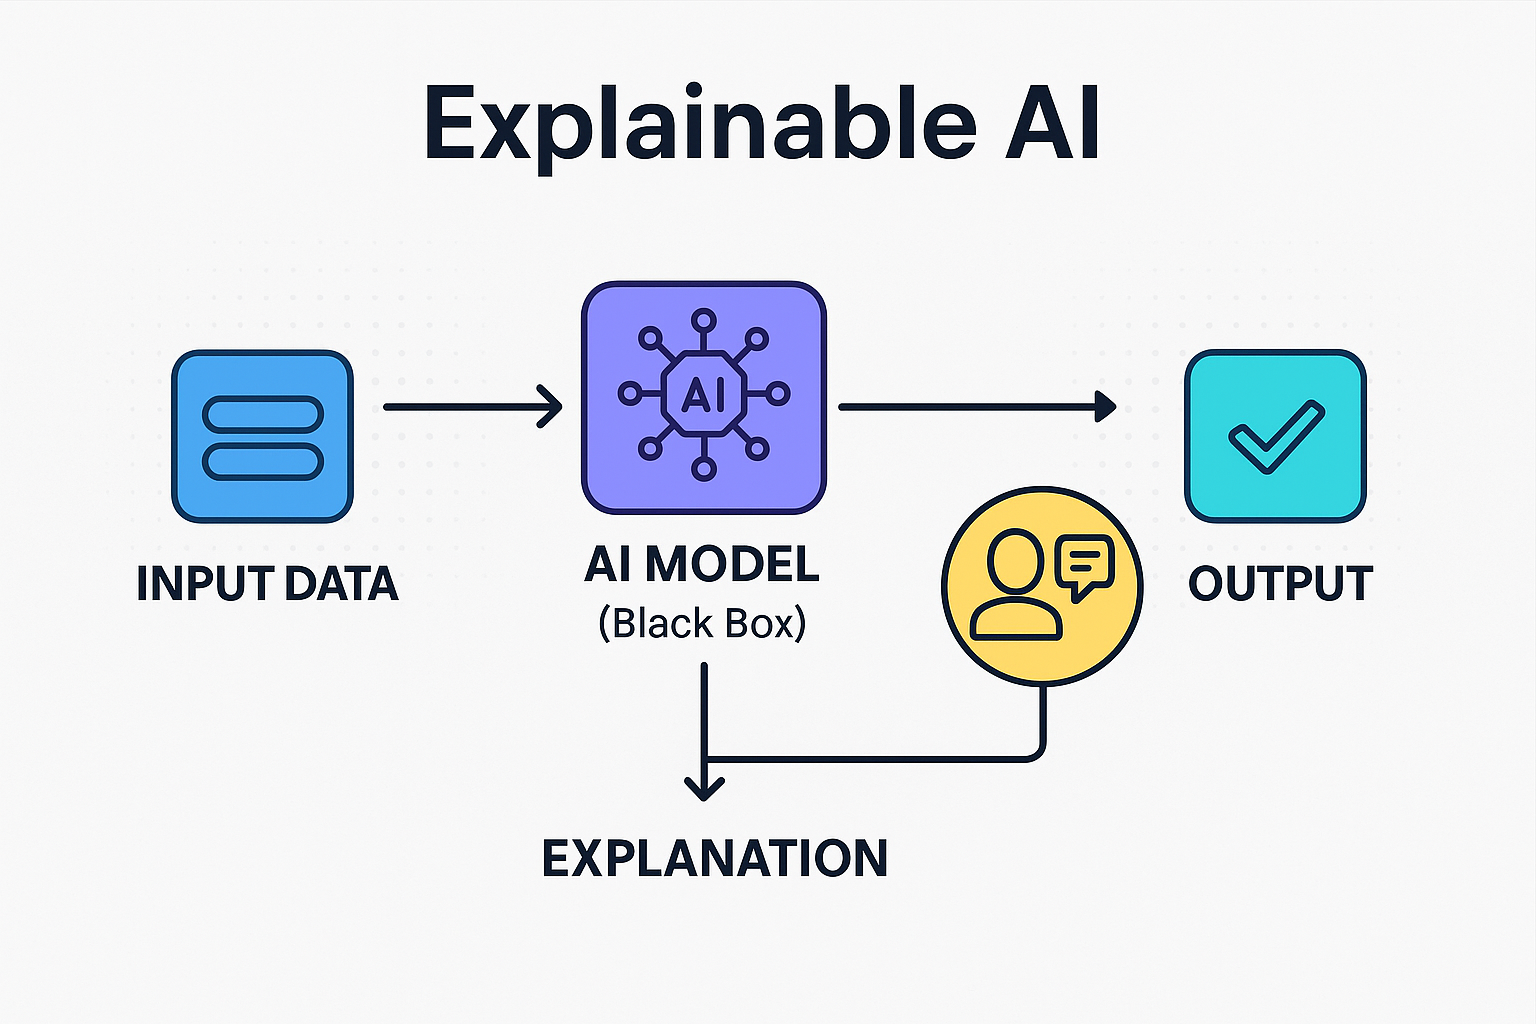
\includegraphics[width=0.6\textwidth]{images/chapter_02/img_08.png}
    \caption{Thuật toán diễn giải mô hình - Explainable AI}
    \label{fig:nlp}
\end{figure}

\noindent
Trong bài toán phân loại văn bản, thuật toán XAI được sử dụng để xác định những từ, token nào trực tiếp góp phần cho kết quả dự đoán, tức là mức độ ảnh hưởng của từ đó đối với kết quả mà mô hình dự đoán được. Ví dụ, trong đồ án này, khi mô hình dự đoán văn bản đó thuộc về lớp AI thì thuật toán sẽ trực tiếp xác định từ hay token nào trong văn bản đó
đóng góp đáng kể cho kết quả dự đoán. Nhờ vậy, kết quả của mô hình không những thể hiện dưới dạng nhãn dự đoán mà còn có thể cung cấp thông tin lý do vì sao lại đưa ra kết quả dự đoán đó. Nhờ đó, XAI hỗ trợ rất tốt trong việc phân tích lỗi và đánh giá các đặc trưng mô hình đã sử dụng trong quá trình phân loại.

\subsection{Thuật toán Integrated Gradients}
Thuật toán Integrated Gradients (IG) là một thuật toán XAI, sử dụng để xác định mức độ đóng góp của từng token so với kết quả dự đoán của mô hình. Phương pháp này sử dụng đạo hàm (gradient) của mô hình để phân tích mức độ ảnh hưởng của dữ liệu đầu vào đến đầu ra, tức là xem đầu ra của mô hình như thế nào khi thay đổi nhỏ đầu vào.

\vspace{\baselineskip}
\noindent
Ý tưởng chính của thuật toán này là xác định mức độ ảnh hưởng của từng đặc trưng dữ liệu đầu vào so với kết quả đầu ra của mô hình. Cách thức hoạt động của thuật toán như sau, đầu tiên IG sẽ bắt đầu từ đầu vào tham chiếu, tức là điểm xuất phát để thuật toán so với câu thực tế (baselines) và thay đổi dần cho đến dữ liệu thực tế. Tại mỗi bước, IG sẽ theo dõi sự thay đổi trong kết quả
dự đoán của mô hình khi dữ liệu đầu vào thay đổi một chút. Sau khi thực hiện qua tất cả các bước thì thuật toán này sẽ tổng hợp lại các kết quả để xem đặc trưng nào có ảnh hưởng ít nhiều so với kết quả dự đoán.

\setcounter{figure}{8}
\begin{figure}[H]
    \centering
    \[
    IG_i(x) = (x_i - x_i') \times \int_{\alpha=0}^{1} \frac{\partial F_i(x' + \alpha (x - x'))}{\partial x_i} \, d\alpha
    \]
    \caption{Công thức tích phân gradient tích hợp của thuật toán Integrated Gradients}
    \label{fig:integrated_gradients}
\end{figure}

\vspace{-0.3cm}
\noindent
Trong đó:
\begin{itemize}
    \item $x$: dữ liệu thực tế cần giải thích.
    \item $x'$: baseline.
    \item $F$: đầu ra của mô hình.
    \item $x_i$: đặc trưng thứ $i$.
    \item $IG_i(x)$: mức độ đóng góp của đặc trưng thứ $i$.
\end{itemize}

\noindent
Trong công thức trên, \(x_i - x_i'\) thể hiện sự khác biệt giữa đặc trưng thứ \(i\) của dữ liệu thực tế so với đặc trưng tương ứng của dữ liệu baseline mà ta đang xét. Ngoài ra, phần đạo hàm  \(\frac{\partial F_i}{\partial x_i}\) cho biết đầu ra của mô hình thay đổi như thế nào khi mà thuật toán thay đổi nhỏ đặc trưng thứ \(i\). Thay vì 
tính toán mức độ ảnh hưởng tại một thời điểm, thuật toán IG sẽ tính toán mức độ thay đổi này tại nhiều điểm trong quá trình đi từ baseline cho đến dữ liệu thực tế và tổng hợp các giá trị vừa tính được qua phép tích phân với $\alpha$ chạy từ 0 đến 1. Trong đó, 0 ở đây tức là vẫn đang ở baseline, 0.5 thì tức là đang ở giữa baseline và dữ liệu thực tế và 1 
đang ở ngay dữ liệu thực tế. Kết quả \(IG_i(x)\) cho biết mức độ đóng góp đặc trưng thứ \(i\) đối với kết quả dự đoán, giá trị càng lớn thì càng ảnh hưởng lớn đối với kết quả dự đoán. Nếu giá trị là dương, thì đặc trưng đang có xu hướng nghiêng ủng hộ phía lớp được dự đoán, còn giá trị âm thì ngược lại.

\vspace{\baselineskip}
\noindent
Ví dụ như trong đồ án phân loại văn bản AI này, các đặc trưng đầu vào đã được biểu diễn dưới dạng embedding của các token trong chuỗi văn bản. Do đó, thuật toán IG sẽ được sử dụng để xác định mức độ đóng góp của từng token đối với kết quả dự đoán của mô hình BamiBERT, những token có mức độ đóng góp lớn thì có ảnh hưởng lớn đến kết quả do mô hình BamiBERT dự đoán,
mức độ ảnh hưởng đó được tính thành một điểm được gọi là điểm đóng góp (Attribution Score).

\subsection{Attribution trong bài toán phân loại văn bản}
Attribution tức là mức độ đóng góp của các đặc trưng đầu vào đối với một kết quả cụ thể mà mô hình tạo ra. Cụ thể, đối với mô hình BamiBERT thì các đặc trưng này tương ứng với từng token trong chuỗi văn bản đang xét. Thông qua thuật toán IG, mỗi token sẽ được gán giá trị điểm đóng góp (Attribution Score) để biết được mức độ ảnh hưởng của token đó đối với kết quả dự đoán.

\vspace{\baselineskip}
\noindent
Trong bài toán phân loại văn bản AI, nếu attribution của một token có giá trị dương thì token đó có xu hướng hỗ trợ cho kết quả dự đoán của lớp đang xét, còn nếu token có giá trị âm thì ngược lại. Ngoài ra, độ lớn tuyệt đối của một token càng lớn thì token đó càng ảnh hưởng mạnh đến kết quả dự đoán của lớp mục tiêu. Nhờ vậy mà cái việc trực quan hóa khả năng diễn giải sẽ rất dễ 
hiểu cho người dùng.

\section{Mô hình ngôn ngữ lớn và ứng dụng trong hệ thống}
\subsection{Mô hình ngôn ngữ lớn (Large Language Model)}
Mô hình ngôn ngữ lớn (Large Language Model - LLM) là một loại mô hình AI được huấn luyện trên lượng lớn dữ liệu văn bản, có khả năng biểu diễn, đọc hiểu, xử lý và tạo ra văn bản bằng ngôn ngữ tự nhiên giống như con người, ví dụ như mô hình GPT, Gemini, Ollama,\dots Thông qua quá trình huấn luyện, mô hình LLM có khả năng nắm bắt, học được mối quan hệ giữa các từ, cấu trúc câu và ngữ cảnh,
từ đó có thể thực hiện nhiều tác vụ như là đọc và trả lời câu hỏi, dịch, tóm tắt văn bản hay là sinh nội dung.

\begin{figure}[H]
    \centering
    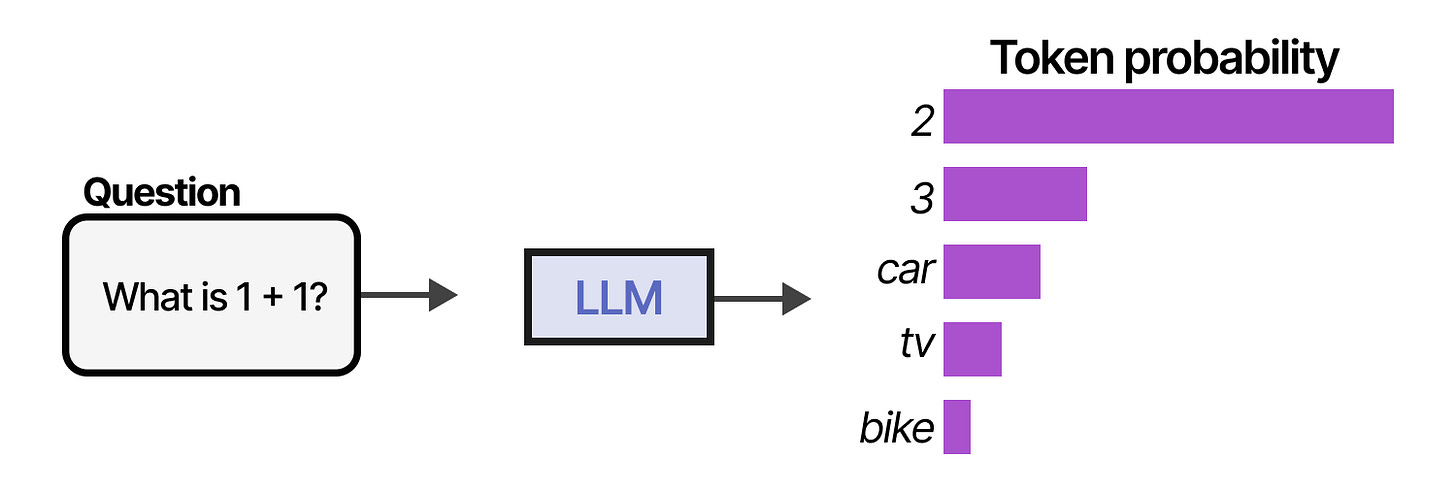
\includegraphics[width=0.8\textwidth]{images/chapter_02/img_10.jpg}
    \caption{Mô hình ngôn ngữ lớn - Large Language Model (LLM)}
    \label{fig:nlp}
\end{figure}

\noindent
Phần lớn các mô hình LLM đều hoạt động dựa trên kiến trúc Transformer, sử dụng cơ chế Self-Attention để khai thác tốt ngữ cảnh trong câu. Đối với quá trình sinh văn bản, LLM sẽ dự đoán token tiếp theo bằng cách tính xác suất của các token tiếp theo dựa trên các token hiện có và lựa chọn token dựa trên phân phối xác suất. Sau đó, token sẽ được thêm vào trong câu và quá trình này sẽ được lặp lại
cho tới khi câu được hoàn thiện. Ngoài ra, khác với các mô hình được xây dựng dựa trên một tác vụ cụ thể thì LLM có khả năng thực hiện nhiều nhiệm vụ khác nhau dựa yêu cầu do người dùng cung cấp dưới dạng prompt, nhờ đó mà mô hình có khả năng thực hiện nhiều nhiệm vụ khác nhau mà không cần phải huấn luyện lại mô hình từ đầu ứng với nhiệm vụ khác nhau.

\subsection{Ứng dụng LLM trong ứng dụng giải thích kết quả}
Trong các hệ thống AI hiện nay, thông thường các kết quả dự đoán của mô hình thường được biểu diễn dưới dạng nhãn, xác suất hoặc các giá trị định lượng thì sẽ gây khó hiểu cho người dùng trong việc hiểu nguyên nhân dẫn đến kết quả. Do đó, LLM thường được sử dụng bằng cách chuyển các giá trị định lượng đó sang giải thích bằng ngôn ngữ tự nhiên, nhờ vậy mà kết quả hệ thống sẽ trở nên minh bạch, dễ hiểu
hơn cho người dùng.

\begin{figure}[H]
    \centering
    
\includegraphics[width=0.5\textwidth]{images/chapter_02/img_11.jpg}
    \caption{Mô hình ngôn ngữ lớn (Gemini)}
    \label{fig:nlp}
\end{figure}

\noindent
Trong đồ án phân loại văn bản AI, IG được sử dụng để xác định mức độ ảnh hưởng, đóng góp của các token cho kết quả dự đoán của mô hình BamiBERT. Tuy nhiên, các giá trị số thường rất khó giải thích và khó hiểu cho người dùng. Do đó, trong đồ án này đã quyết định sử dụng mô hình Gemini để sử dụng và phân tích những giá trị định lượng đó, tạo ra những lời giải thích mà chỉ phụ thuộc vào các giá trị mà thuật toán, mô
hình đã tính ra bằng ngôn ngữ tự nhiên nhằm giúp cho người dùng hiểu được những thành phần nào trong văn bản có ảnh hưởng đến kết quả phân loại.
% !TEX root = main.tex
\chapter{Dữ liệu và phương pháp xây dựng hệ thống}

\section{Tổng quan hệ thống}

\begin{figure}[H]
    \centering
    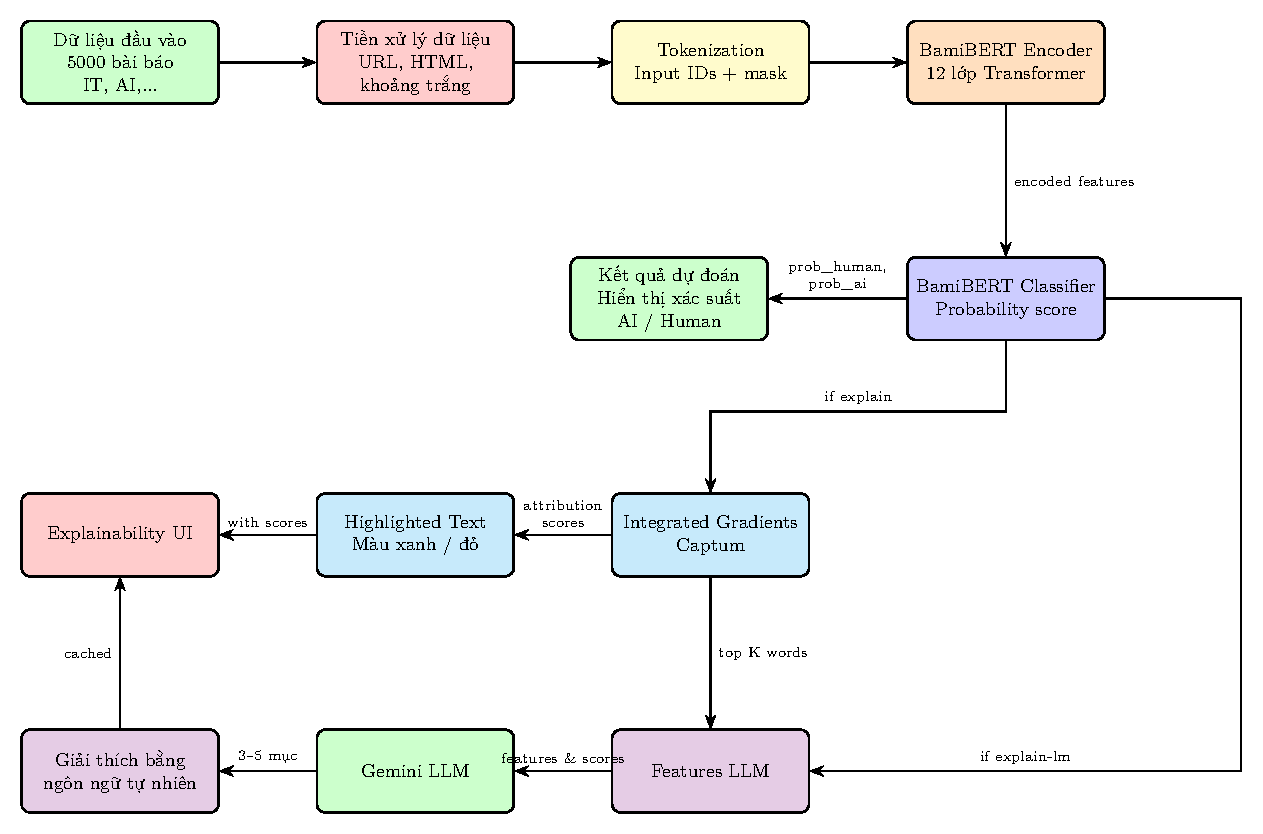
\includegraphics[width=\textwidth]{figures/chapter_03/system_architecture.pdf}
    \caption{Kiến trúc hệ thống}
    \label{fig:system_architecture}
\end{figure}

Trong hệ thống trên, dữ liệu đầu vào tập trung vào các bài báo tiếng Việt chuyên về lĩnh vực công nghệ thông tin (IT), AI hay là các thiết bị công nghệ hiên đại. Dữ liệu sau đó được tiền xử lý bằng cách loại bỏ các URL, HTML, và khoảng trắng thừa, dữ liệu đã được làm sạch
sẽ được đưa vào quá trình token hóa, để ánh xạ mỗi từ sang các chỉ số đầu vào (input IDs) và mặt nạ (mask). Tiếp theo, các token này sẽ được được vào mô hình BamiBERT để embedding, tức là chuyển các token thành các vector đặc trưng rồi bắt đầu quá trình huấn luyện. Đầu ra
của mô hình chính là xác suất dự đoán của văn bản dựa vào hai lớp, Human hay là AI.

\vspace{\baselineskip}
\noindent
Ngoài ra, hệ thống còn có khả năng giải thích kết quả do mô hình dự đoán bằng cách sử dụng thuật toán Integrated Gradients, thuật toán này sẽ tính điểm đóng góp cho từng token của đoạn văn bản, dựa vào điểm đóp góp đó thì hệ thống sẽ hiển thị giao diện bằng cách highlight các từ đó theo
các màu tương ứng với hai lớp, cụ thể màu đó là AI và màu xanh là người viết, độ sáng của các màu thể hiển mức độ đóng góp, ảnh hưởng đối với kết quả dự đoán, màu càng đậm thì càng ảnh hưởng lớn đối với kết quả dự đoán.

\vspace{\baselineskip}
\noindent
Tiếp theo để hệ thống có khả năng giải thích bằng ngôn ngữ tự nhiên, hệ thống đã sử dụng một mô hình LLM, đó là Gemini, với sự ràng buộc yêu cầu (prompt) dựa trên các từ có điểm đóng góp cao từ thuật toán IG, và các chỉ số đo lường ví dụ như mật độ dấu câu, độ dài câu,\dots Sau đó câu lệnh sẽ được mô hình
Gemini xử lý và trả về kết quả giải thích bằng ngôn ngữ tự nhiên, kết quả này sẽ được hiển thị trên giao diện của người dùng.

\section{Thu thập và xây dựng dữ liệu}
\subsection{Nguồn dữ liệu}
Nguồn dữ liệu được thu thập trong đồ án chủ yếu là đến từ các trang báo, bài viết tiếng Việt thuộc lĩnh vực công nghệ thông tin, AI hay các thiết bị công nghệ hiện đại, \dots Việc lựa chọn một lĩnh vực cụ thể nhằm đảm bảo dữ liệu có tính thống nhất về chủ đề, đồng thời hạn chế về sự khác biệt về chủ đề có ảnh hưởng đến quá trình học của mô hình. Ngoài 
ra, lĩnh vực công nghệ có lượng lượng bài báo, nội dung thường xuyên đăng tải liên tục trực tuyến, thường có sự thay đổi về công nghệ, thuật ngữ chuyên môn, tên sản phẩm và tên công nghệ, \dots Điều này tạo nên tính đa dạng về dữ liệu vì cách diễn đạt, cấu trúc bài viết khác nhau.

\begin{figure}[H]
    \centering
    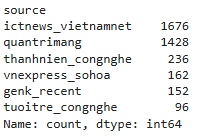
\includegraphics[width=0.4\textwidth]{images/chapter_03/img_13.png}
    \caption{Các nguồn dữ liệu thu thập}
    \label{fig:nlp}
\end{figure}

\vspace{\baselineskip}
\noindent
Phần lớn các bài báo, tin tức được thu thập từ các nguồn uy tín, tên miền rõ ràng, đều là các trang bài báo công nghệ phổ biến ở Việt Nam, bao gồm VnExpress, GenK, Thanh Niên Công Nghệ,\dots Các bài báo được thu thập từ các nguồn này đều có nội dung liên quan đến lĩnh vực công nghệ thông tin, AI hay các thiết bị công nghệ hiện đại,\dots Các nguồn này
được lựa chọn dựa trên mức độ phổ biến, ổn định và độ tin cậy của các trang tin tức Việt Nam. Nhờ vậy mà dữ liệu có nguồn gốc rõ ràng và phù hợp với phạm vi nghiên cứu.


\subsection{Thu thập dữ liệu văn bản Human}
Dữ liệu các bài báo, văn bản Human được thu thập tập trung vào các lĩnh vực công nghệ thông tin, trí tuệ nhân tạo, thiết bị công nghệ hiện đại như đã trình bày ở mục 3.2.1. Mục đích của quá trình này là để xây dựng một bộ dữ liệu bài báo, văn bản được viết và xuất bản bởi con người, lấy làm cơ sở để mô hình học cách phân biệt nội dung giữa con người hay AI tạo ra. Quá trình 
thu thập dữ liệu được tự động hóa bằng cách truy cập các trang tin tức và trích xuất nội dung từ các bài báo, bài viết phù hợp. Đối với mỗi bài viết, các phần quan trọng như URL, nguồn, tên tác giả và ngày xuất bản sẽ được lưu trữ nhằm thể hiện các bài báo đó có nguồn rõ ràng, minh bạch và nội dung của bài báo đó. Các phần không liên quan đến nội dung như quảng cáo, menu hay 
các thành phần giao diện web sẽ được loại bỏ để đảm bảo dữ liệu thu được chỉ tập trung vào các nội dung cần thiết.

\begin{figure}[H]
    \centering
    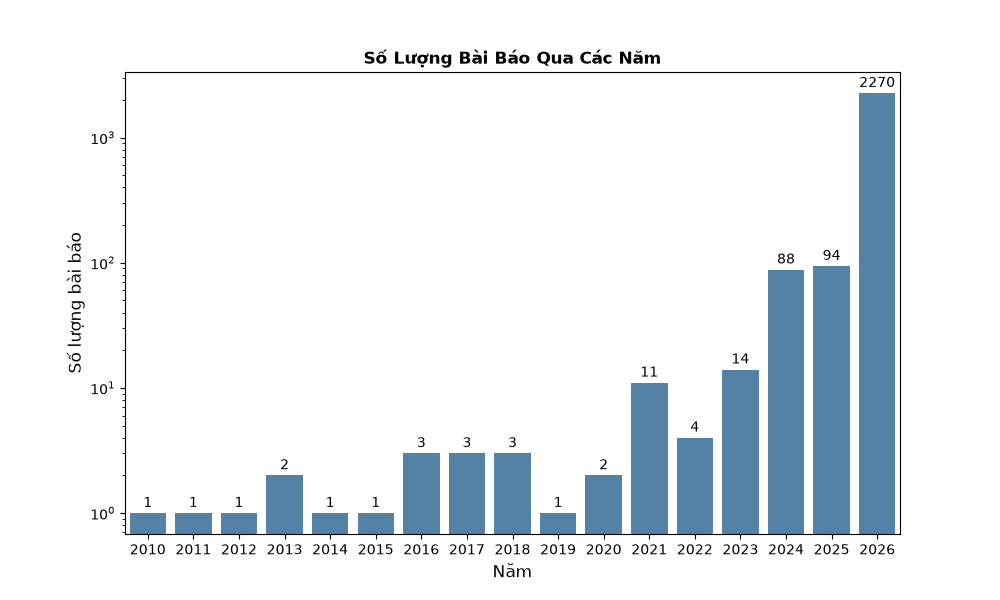
\includegraphics[width=1.0\textwidth]{images/chapter_03/img_14.png}
    \caption{Các bài báo văn bản thu thập qua các năm}
    \label{fig:nlp}
\end{figure}

\vspace{\baselineskip}
\noindent
Như đã thấy ở Hình 14, dữ liệu được thu thập từ các bài báo, tin tức nằm trong khoảng từ năm 2010 cho đến năm 2026 và tập trung hầu hết vào năm 2026 với tổng cộng là 2.270 bài. Nguyên nhân là trong quá trình thu thập dữ liệu, các nguồn tin tức thường cung cấp số lượng bài báo mới hiện nay nhiều hơn so với các bài viết từ các năm trước, ngoài ra thì các bài báo cũ từ các năm trước có 
khả năng truy cập và thu thập bị hạn chế hơn rất nhiều, có thể là do cấu trúc website thay đổi theo thời gian hoặc là do trang lưu trữ dữ liệu các bài báo cũ không còn tồn tại nữa. Do đó, dữ liệu được giữ theo số lượng thực tế thay vì cố gắng thu thập phân bố đồng đều giữa các năm.

\vspace{\baselineskip}
\noindent
Ngoài ra, sẽ có vấn đề là nếu muốn dữ liệu Human là viết hoàn toàn bởi con người, ít ảnh hưởng bởi AI nhất thì tại sao không thu thập dữ liệu từ các năm trước trở xuống, ví dụ như năm 2023, là thời điểm AI chưa phát triển mạnh để các tác giả sử dụng để hỗ trợ khả năng viết bài của họ. Lý do là vì nếu ta chỉ thu thập từ các năm trước, giả sử như năm 2023 trở về trước, thì dữ liệu sẽ bị hạn chế về số lượng 
và tính đa dạng của nó, đó là yếu tổ sự chuyển dịch theo thời gian, giả sử như năm 2023, các bài viết chưa có đề cập đến các chủ đề như Claude, OpenClaw, Gwen, \dots Trong khi các bài báo hiện nay thì lại rất nhiều, điều đó vô tình khiến một vấn đề lớn là khi sau này hệ thống mà triển khai thì khi mà đưa một bài báo mà mô hình chưa thấy chủ đề đó bao giờ thì sẽ khó mà phân loại được, vì bản thân mô hình học sâu,
mô hình được sử dụng trong đồ án ngoài khả năng học cấu trúc câu, thì nó còn học thêm từ vựng, chủ đề và ngữ cảnh xuất hiện trong câu, do đó khả năng tổng quát hóa của mô hình sẽ trở nên kém hơn nếu đem đi triển khai thực tế. Do đó, đồ án quyết định xây dựng dữ liệu qua các năm, từ năm 2010 đến 2026 và tập trung hầu hết từ năm 2024 - 2026 để đảm bảo tính đa dạng về chủ đề, đa dạng hóa các nguồn và sát với dữ liệu
thực tế để đi vận hành triển khai hệ thống. 

\subsection{Xây dựng dữ liệu AI}
Dữ liệu AI được xây dựng dựa trên các mô hình ngôn ngữ lớn (LLM) nhằm tạo ra các mẫu bài báo, văn bản phục vụ cho viết huấn luyện mô hình phân biệt giữa văn bản do con người viết hay AI tạo ra. Dữ liệu bài báo AI được xây dựng bằng cách đưa ra chủ đề kết hợp với yêu cầu hoàn chỉnh để mô hình LLM tạo ra các bài báo, tức là sẽ chọn các chủ đề liên quan đến lĩnh vực đồ án, ví dụ như trí tuệ nhân tạo, smartphone, ứng dụng công nghệ, \dots Sau
đó, đưa ra các yêu cầu cụ thể về độ dài, cấu trúc bài viết, số lượng đoạn văn để đảm bảo giống như các bài báo từ con người, có nguồn rõ ràng để cho mô hình LLM sinh ra. 

\vspace{\baselineskip}
\noindent
Ở phạm vi đồ án, mô hình LLM sử dụng là bao gồm Gemini và DeepSeek, vì lý do là khi sử dụng các mô hình khác, ví dụ như ChatGPT hay Claude thì sẽ tốn token và tốn rất nhiều chi phí mà ngân sách thì hạn hẹp cho nên lựa chọn hai mô hình đó để sinh bài báo, văn bản là cách tối ưu
cho phạm vi đồ án. Tuy vậy, vẫn có một nhược điểm đó là nếu giới hạn các mô hình sinh văn bản như vậy thì khi mà triển khai thì người dùng vẫn có thể sử dụng các mô hình ngôn ngữ khác tốt hơn để sinh bài báo, ví dụ như các mô hình Opus 5 hay Fable 5 của Claude với khả năng viết lách giống như con người hơn thì hệ thống sẽ vẫn khó để phân biệt loại bài báo đó là do con người hay AI tạo nên.

\subsection{Xây dựng dữ liệu AI-rewritten}
Dữ liệu AI-rewritten, chính là dữ liệu AI tạo ra dựa trên dữ liệu con người, tức là sử dụng AI để viết lại, thay đổi cấu trúc và văn phong dựa trên dữ liệu do con người, từ các nguồn uy tín. Mục đích của quá trình này là tạo ra các bài báo, văn bản mô phỏng trường hợp mà các bài viết ban đầu do con người viết nhưng được sử dụng AI để diễn đạt lại, và bài viết đó vẫn chứa chất xám của con người. Trong thực tế, có
một số người lợi dụng các công cụ AI để viết lại những văn bản được tạo bởi con người nhằm làm cho nội dung khó bị phát hiện hơn, với mục đích sử dụng bài viết, chất xám của người khác để thay đổi cấu trúc, văn phong làm bài viết của mình. 

\vspace{\baselineskip}
\noindent
Trong các trường hợp đó thì nội dung, thông tin chính vẫn còn được giữ lại, trong khi cách sử dụng từ ngữ, cấu trúc câu hay phong cách diễn đạt lại được thay đổi. Điều này vô tình dẫn đến một thách thức lớn đối với các hệ thống phát hiện văn bản AI, lý do đơn giản là bởi vì các văn bản do AI viết lại không còn mang những đặc điểm rõ ràng của các văn bản do AI tạo hoàn toàn từ đầu.

\vspace{\baselineskip}
\noindent
Để mô phỏng trường hợp đó thì trong đồ án, em đã xây dựng dữ liệu AI-rewritten dựa trên các bài báo, bài viết thuộc lớp Human đã thu thập. Quá trình tạo dữ liệu như sau, nội dung của bài báo từ lớp Human sẽ được đưa vào các mô hình LLM, cụ thể trong đồ án thì các mô hình LLM vẫn giống như cách xây dựng tập dữ liệu AI tự sinh hoàn toàn, đó là mô hình Gemini và Claude, kết hợp với yêu cầu (prompt) viết lại với
cấu trúc câu thay đổi, độ dài văn bản không thay đổi quá nhiều, thay đổi từ vựng và cách diễn đạt. Sau đó các bài báo được mô hình LLM sinh ra và sẽ được gán vào lớp AI với một thuộc tính phân biệt là "rewritten".


\subsection{Cấu trúc và tổ chức dữ liệu}
Dữ liệu được tổ chức dưới dạng bảng, mỗi hàng là một mẫu bài báo tương ứng với các đặc trưng liên quan đến quá trình phụ vụ huấn luyện mô hình. Tập dữ liệu (Dataset) được thiết kế nhăm phân biệt các bài báo do con người viết và do mô hình ngôn ngữ lớn góp phần tạo ra.

\begin{figure}[H]
    \centering
    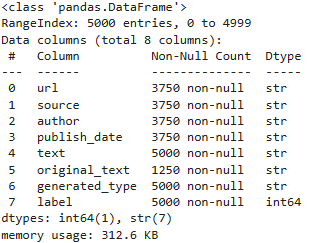
\includegraphics[width=0.5\textwidth]{images/chapter_03/img_15.png}
    \caption{Cấu trúc dữ liệu của hệ thống}
    \label{fig:nlp}
\end{figure}

\vspace{\baselineskip}
\noindent
\begin{table}[H]
    \centering
    \begin{tabular}{>{\bfseries}p{3.0cm}p{2.2cm}p{8.2cm}}
        \toprule
        Trường & Loại & Ý nghĩa \\
        \midrule
        \texttt{url} & \texttt{Metadata} & Nguồn URL của các bài báo \\
        \texttt{source} & \texttt{Metadata} & Tên miền của các bài báo. \\
        \texttt{author} & \texttt{Metadata} & Tên tác giả của bài báo. \\
        \texttt{publish\_date} & \texttt{Metadata} & Ngày xuất bản bài báo. \\
        \texttt{text} & \texttt{Đặc trưng đầu vào} & Nội dung văn bản được sử dụng cho quá trình huấn luyện và dự đoán. \\
        \texttt{original\_text} & \texttt{Dữ liệu tham chiếu} & Văn bản gốc trước khi được mô hình ngôn ngữ viết lại. \\
        \texttt{generated\_type} & \texttt{Metadata} & Phương tháp tạo ra bài báo. \\
        \texttt{label} & \texttt{Nhãn} & Nhãn phân loại, biểu thị văn bản Human hoặc AI. \\
        \bottomrule
    \end{tabular}
    \caption{Mô tả các trường trong tập dữ liệu}
    \label{tab:data_structure}
\end{table}

\noindent
Như vậy, bộ dữ liệu được tổ chức với trường thông tin được sử dụng để lưu trữ nội dung văn bản, nhãn phân loại và các thông tin liên quan đến nguồn dữ liệu. 
Ngoài ra, \texttt{text} là nội dung bài báo và \texttt{label} là thành phần chính để phục vụ cho quá trình mô hình học và dự đoán, còn các trường còn lại được
sử dụng cho mục đích phân tích và khai thác sâu vào dữ liệu.

\subsection{Phân bố dữ liệu}
Như ta đã thấy ở Hình 15, dữ liệu là tổng cộng gồm có 5000 mẫu. Trong đó, cột \texttt{label} được chia thành hai lớp có số lượng mẫu bằng nhau, đó là lớp AI và Human có
số lượng mẫu đều là 2500 mẫu.

\begin{figure}[H]
    \centering
    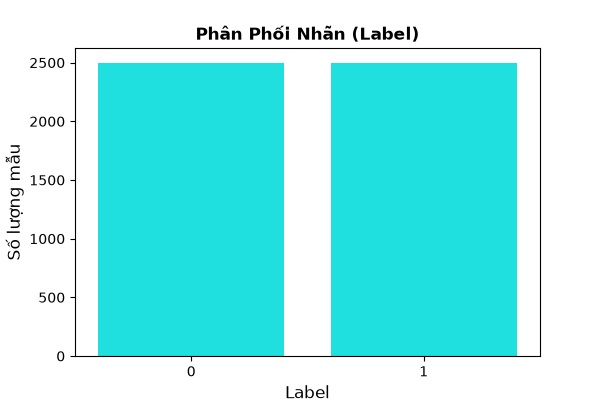
\includegraphics[width=0.8\textwidth]{images/chapter_03/img_16.png}
    \caption{Phân bố nhãn \texttt{label}}
    \label{fig:nlp}
\end{figure}

\noindent
Ngoài ra, trường \texttt{generated\_type} cũng đã phân bố đều, với ba thành phần đó là Human, Generated (bài báo do AI sinh ra hoàn toàn từ đầu), Rewritten (bài báo do AI viết
lại từ bài báo của con người, có nguồn rõ ràng). Dữ liệu cũng được tổ chức, phân bố đều với Human chiếm tới 2500 mẫu và hai thành phần còn lại, mỗi phần tương ứng 1250 mẫu.

\begin{figure}[H]
    \centering
    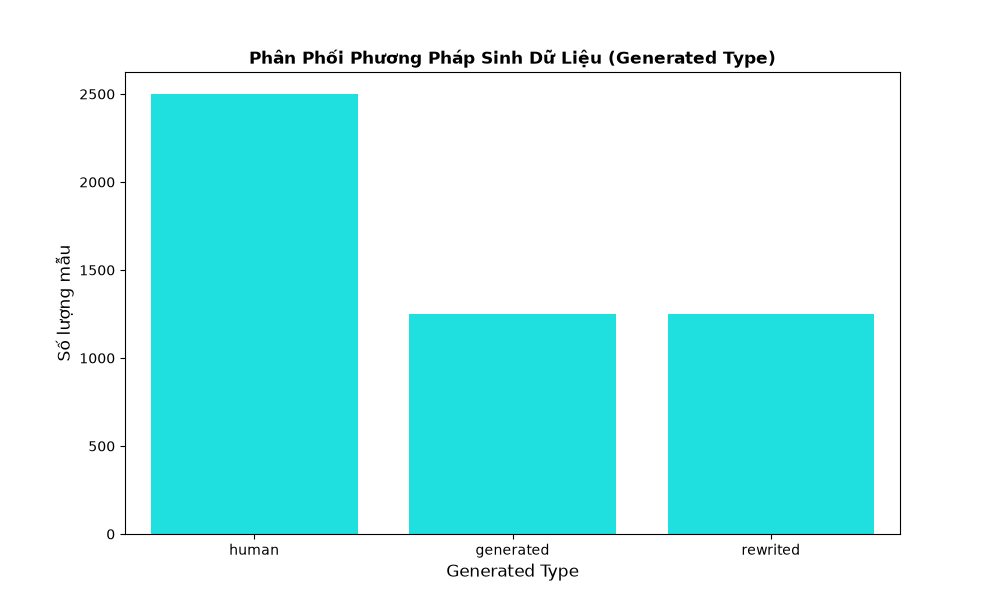
\includegraphics[width=0.9\textwidth]{images/chapter_03/img_17.png}
    \caption{Phân bố phương pháp tạo sinh dữ liệu}
    \label{fig:nlp}
\end{figure}

\noindent
Bên cạnh sự phân bố nhãn và phương pháp sinh dữ liệu, độ dài văn bẳn cũng là một yếu tố, đặc điểm cần đáng được xem xét trong quá trình phân tích toàn bộ dữ liệu. Sự khác biệt độ dài giữa
các nhóm văn bản có thể thể phản ánh những đặc điểm khác nhau trong quá trình biên soạn và tạo nội dung, đồng thời đánh giá được mức độ tương đồng về mặt độ dài giữa dữ liệu AI và Human.

\begin{figure}[H]
    \centering
    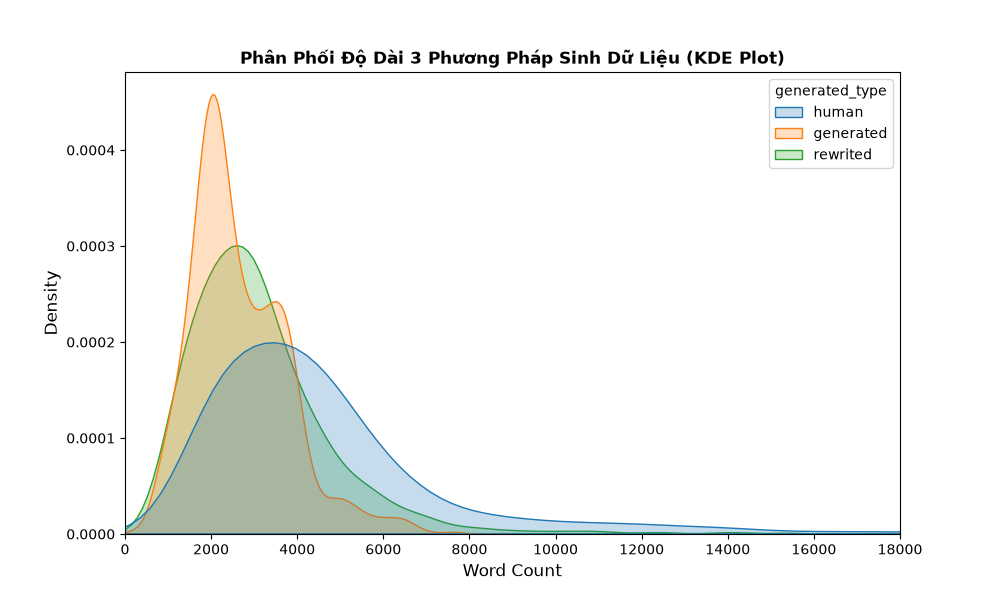
\includegraphics[width=1.0\textwidth]{images/chapter_03/img_18.png}
    \caption{Phân bố độ dài của các phương pháp tạo sinh dữ liệu}
    \label{fig:nlp}
\end{figure}

\noindent
Biểu đồ ước lượng mật độ nhân (Kernel Density Estimate - KDE) là một loại biểu đồ được sử dụng để trực quan hóa sự phân phối của một tập dữ liệu liên tục. Ở hình 18 trên, biểu đồ thể hiện mật dộ của phân
phối số lượng từ dựa trên ba phương pháp sinh dữ liệu. 

\vspace{\baselineskip}
\noindent
Ta có thể thấy nhóm sử dụng AI để tự sinh dữ liệu từ đầu (Generated) có mật độ cao nhất, nằm trong khoảng 2.000 - 3.500 từ và một số ít tập trung vào khoảng gần 4.000 - 4.500 từ ở mỗi bài. Điều này dữ liệu AI sinh văn bản
từ đầu trong đồ án có xu hướng tuân theo một khuôn mẫu về độ dài, ít biến động và phần lớn độ dài của văn bản khá là tương đồng.

\vspace{\baselineskip}
\noindent
Ngoài ra, nhóm Human có mật độ phân bố trải rộng rõ rệt hơn so với hai nhóm còn lại, khoảng 3.500 - 4.500 từ mỗi bài. Ở phía bên phải còn tồn tại rất nhiều văn bản trải rộng, tức là còn tồn tại nhiều văn bản có độ dài lớn
hơn so với mặt bằng chung. Điều này phản ánh tính đa dạng của nhóm Human khi xây dựng các nội dung bài báo so với hai nhóm còn lại. 

\vspace{\baselineskip}
\noindent
Tuy vậy, mật độ phân phối độ dài của ba nhóm có một phần chồng lấn, tập trung từ 2.000 - 4.000 từ khá nhiều. Cho thấy được độ dài cũng chưa phải là một đặc trưng đủ mạnh để mô hình đưa ra quyết định, còn phải phụ thuộc thêm ngữ nghĩa,
cấu trúc câu và từ vựng của từng loại bài báo.


\section{Tiền xử lý dữ liệu}
\subsection{Làm sạch và chuẩn hóa văn bản}
Sau khi đã phân tích, tìm hiểu cấu trúc, sự phân bố dữ liệu thì ta sẽ thực hiện quát trình làm sạch dữ liệu. Trong đồ án, quá trình làm sạch dữ liệu gồm ba bước: loại bỏ HTML, URL và loại bỏ khoảng trắng đầu và cuối của chuỗi, lý do là vì các mã code hay đường dẫn thì nó
không phản ánh cách viết của người hay AI và khoảng trắng chỉ làm tốn tài nguyên xử lý mà không mang lại giá trị ngữ nghĩa.

\begin{lstlisting}[style=pythoncode]
def clean_text(text):
    text = BeautifulSoup(text, 'html.parser').get_text()
    text = re.sub(r'http\S+|www\S+', '', text)
    text = re.sub(r'\s+', ' ', text).strip()
    return text
\end{lstlisting}

\captionof{listing}{Hàm làm sạch dữ liệu}

\begin{figure}[H]
    \centering
    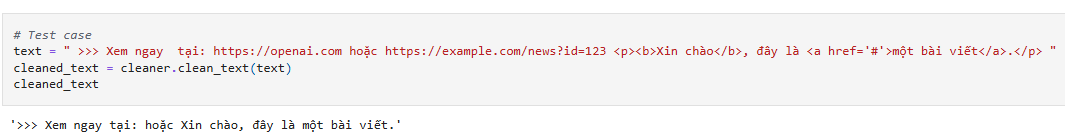
\includegraphics[width=1.0\textwidth]{images/chapter_03/img_19.png}
    \caption{Đoạn văn bản sau khi đã làm sạch}
    \label{fig:nlp}
\end{figure}

\noindent
Tuy nhiên vẫn có một điều cần làm rõ là trong đồ án phân loại văn bản AI này thì vẫn giữ nguyên dấu câu, chữ hoa, chữ thường, định dạng từ và các biểu cảm của văn bản gốc. Lý do là vì các thành phần đó là tín hiệu cực mạnh để phân biệt văn bản do người viết hay do AI tạo ra, các
thành phần đó cung cấp thông tin về phong cách viết, cấu trúc câu và cách sử dụng ngôn ngữ cho mô hình phân loại. Nhưng em vẫn không thể khẳng định đây là những đặc điểm chính xác luôn có khả năng phân biệt giữa con người viết hay do AI tạo ra. Bởi vì một tác giả họ có thể có khả 
năng viết một bài báo rất mạch lạc, tuân thủ nguyên tắc và sử dụng dấu câu một cách chính xác, trong khi các mô hình LLM hiện nay cũng có khả năng tạo ra văn bản giống như con người. Vì vậy, đồ án đã không loại bỏ những thành phần này mà giữ nguyên chúng để mô hình có thể tự học mức
độ đóng góp của từng đặc điểm dựa trên dữ liệu huấn luyện, thay vì áp đặt một đặc điểm nào đó chắc chắn là của Human hay là AI, tức là ví dụ như văn bản có nhiều dấu câu thì mình dự đoán đó là AI hay văn bản có lỗi chính tả là của Human thì các giả định này không phải lúc nào cũng đúng.

\subsection{Tokenization}
Sau bước làm sạch dữ liệu, bước tiếp theo là tokenization, tức là token hóa, nhằm chuyển đổi văn bản từ dạng chuỗi ký tự sang các đơn vị nhỏ hơn được gọi là token, token ở đây có thể là ký tự, thành phần của từ đó hay chính từ đó. Trong đồ án, em sử dụng bộ token hóa là của mô hình BamiBERT thông qua thư viện HuggingFace Transformer.

\vspace{\baselineskip}
\begin{lstlisting}[style=pythoncode]
from transformers import AutoTokenizer
tokenizer = AutoTokenizer.from_pretrained("Qualcomm-AI-Research/BamiBERT")
\end{lstlisting}

\captionof{listing}{Định nghĩa bộ token hóa BamiBERT}

\noindent
Bộ token hóa của mô hình BamiBERT sử dụng thuật toán Byte-level Byte Pair Encoding (BBPE), tức là thuật toán có khả năng tách một từ thành token dựa vào các tiêu chí nhất định dựa vào bộ từ vựng mà mô hình đã được huấn luyện, bao gồm từ phổ biến thì sẽ giữ nguyên cả từ (ví dụ: bánh mì $\rightarrow$ bánh\_mì), từ hiếm hoặc từ mới thì sẽ tách thành các thành 
phần con (subwords) và các từ hoàn toàn chưa biết thì sẽ được tách thành ký tự đơn.

\begin{lstlisting}[style=pythoncode]
MAX_LENGTH = 1024
it_ai_human_df['tokens'] = it_ai_human_df['cleaned_text'].apply(
    lambda x: tokenizer.tokenizer(
        x,
        max_length=MAX_LENGTH,
        truncation=True,
        padding='max_length',
        return_tensors='pt'
    )
)

# Extract input_ids + attention_mask
it_ai_human_df['input_ids'] = it_ai_human_df['tokens'].apply(lambda x: x['input_ids'][0].tolist())
it_ai_human_df['attention_mask'] = it_ai_human_df['tokens'].apply(lambda x: x['attention_mask'][0].tolist())
\end{lstlisting}

\captionof{listing}{Thực hiện token hóa văn bản}

\vspace{\baselineskip}
Quá trình tokenization sẽ được thực hiện ngay chính cột \texttt{cleaned\_text}, tức là cột chứa các văn bản sau khi đã làm sạch với độ dài tối đa mà bộ token hóa xử lý là 1024 token (\texttt{MAX\_LENGTH}). Nếu mà đoạn văn bản có độ dài vượt quá 1024 token thì sẽ thực hiện cắt đoạn ngay token thứ 1024 đó (truncation), còn các đoạn văn bản mà có độ dài nhỏ hơn 1024 token thì
sẽ chèn thêm các token \texttt{<PAD>} để cho đủ độ dài mà mô hình ban đầu giới hạn cho phép. Sau đó, các token sẽ được ánh xạ thành hai thành phần, đó là \texttt{input\_ids} và \texttt{attention\_mask}.

\vspace{\baselineskip}
\noindent
Trong đó, \texttt{input\_ids} là dãy số đại diện cho các token trong văn bản, ví dụ như các token sau: \texttt{["Sự", "xuất", "hiện", "của", "iPhone", "17e", ...]} thì sẽ ánh xạ
thành \texttt{[2470, 621, 447, 275, 4189, 1377, ...]}, mỗi con số thì sẽ tương ứng với một token trong bộ từ điển của tokenizer BamiBERT. \texttt{attention\_mask} sẽ cho mô hình BamiBERT biết token nào là token thật và token nào là padding, token padding ở đây chính là những token mà tokenizer sẽ chèn vào nếu độ dài của văn bản đó không đủ 1024 token, ví dụ như \texttt{input\_ids} 
gồm các ID của văn bản như sau:\texttt{[101, 2470, 621, 447, 275, 102, 0, 0, 0, ...]} thì \texttt{attention\_mask} sẽ ánh xạ thành \texttt{[1, 1, 1, 1, 1, 1, 0, 0, 0, ...]}. Trong đó 1 tương ứng với token thật, mô hình cần phải chú ý đến và 0 tức là token padding, mô hình sẽ bỏ qua. Hai thành phần đó đóng vai trò quan trọng cho việc phối hợp cùng nhau để cho mô hình học sâu được sử dụng
để huấn luyện có thể xử lý các văn bản có độ dài khác nhau sau khi được padding về cùng kích thước.

\section{Xây dựng và fine-tuning mô hình phân loại}
\subsection{Tạo group ID}
Bởi vì trong quá trình tạo dữ liệu AI-rewritten, em có sử dụng dữ liệu Human đã thu thập được làm văn bản gốc rồi sử dụng LLM để viết lại, nên là phải có một bước ghép các đoạn văn bản có \texttt{original\_text} (AI-rewritten) trùng với lại \texttt{text} (Human) để tránh bị lộ dữ liệu trong quá trình huấn luyện, ví dụ như nếu trong quá trình kiểm tra (test) mà xuất hiện một đoạn văn bản có \texttt{original\_text}
trùng với lại \texttt{text} của đoạn văn bản đó trong quá trình huấn luyện thì mô hình vô tình đã biết trước dữ liệu, điều này dẫn đến khả năng tổng quát hóa của mô hình kém đi.

\begin{figure}[H]
    \centering
    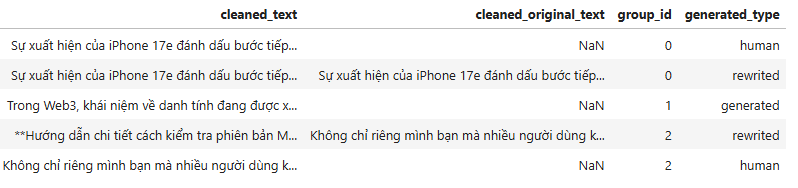
\includegraphics[width=1.0\textwidth]{images/chapter_03/img_20.png}
    \caption{Đoạn văn bản sau đã nhóm theo ID}
    \label{fig:nlp}
\end{figure}

\subsection{Chia tập dữ liệu}
Sau khi đã tạo \texttt{group\_id}, ta sẽ tiến hành chia tập dữ liệu thành ba phần: tập huấn luyện (train), tập xác thực (validation) và tập kiểm thử (test). Việc chia dữ liệu theo \texttt{group\_id} đảm bảo các văn bản có không bị trùng \texttt{original\_text} và \texttt{text} ở nhiều tập dữ liệu. Sau khi chia, dữ liệu 
gồm 3.502 mấu cho tập train, 766 cho tập validation và 732 cho tập test, tức là tỉ lệ xấp xỉ 70/15/15.

\begin{figure}[H]
    \centering
    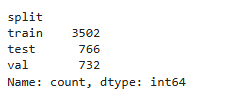
\includegraphics[width=0.4\textwidth]{images/chapter_03/img_21.png}
    \caption{Tỉ lệ tập dữ liệu sau khi chia}
    \label{fig:nlp}
\end{figure}

\subsection{Định nghĩa mô hình phân loại phù hợp với bài toán}

\begin{lstlisting}[style=pythoncode]
class AIContentModel(nn.Module):
    """
    BamiBert Encoder + Classification Head.
    """
    def __init__(self, model_name='Qualcomm-AI-Research/BamiBERT', num_classes=2, dropout=0.1):
        super().__init__()
        self.bert = AutoModel.from_pretrained(model_name)
        hidden_size = self.bert.config.hidden_size # 768 for base 
        self.dropout = nn.Dropout(dropout)
        self.classifier = nn.Linear(hidden_size, num_classes)

    def forward(self, input_ids, attention_mask):
        outputs = self.bert(input_ids=input_ids, attention_mask=attention_mask)

        # [CLS] token represents for first token
        cls_output = outputs.last_hidden_state[:, 0, :]
        x = self.dropout(cls_output)
        logits = self.classifier(x)

        return logits
\end{lstlisting}

\captionof{listing}{Định nghĩa mô hình phân loại}
Trong đồ án, em sẽ tự định nghĩa mô hình phân loại thành một class riêng, mô hình \texttt{AIContentModel}. Đây là mô hình được định nghĩa dựa trên mô hình nền BamiBERT và được thiết kế riêng
cho bài toán phân loại văn bản AI. Kích thước biểu diễn vector sẽ lấy từ mô hình BamiBERT thông qua \texttt{hidden\_size} với 768 chiều. Vector biễu diên của token \texttt{[CLS]} tại vị trí đầu tiên
của chuỗi văn bản được lấy từ \texttt{last\_hidden\_state}, vì đây là nơi mà mô hình BamiBERT lưu toàn bộ các vector biểu diễn của các token sau khi đã đi qua toàn bộ layer của quá trình Encoder.

\vspace{\baselineskip}
\noindent
Sau đó, vector này sẽ đi qua lớp Dropout, là một lớp có khả năng giảm hiện tượng quá khớp (overfitting) bằng cách tắt ngẫu nhiên một số neuron trong quá trình huấn luyện.

\begin{figure}[H]
    \centering
    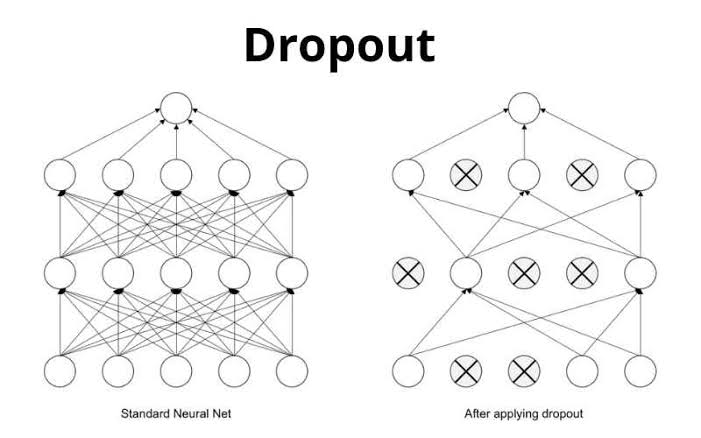
\includegraphics[width=0.7\textwidth]{images/chapter_03/img_22.jpg}
    \caption{Hiện tượng dropout trong mạng neuron}
    \label{fig:nlp}
\end{figure}

\vspace{\baselineskip}
\noindent
Cuối cùng, các vector đó sẽ được đưa vào lớp Classification Head để ánh xạ vector 768 chiều sang 2 chiều, 2 chiều ở đây sẽ mang giá trị là logit tương ứng với 2 lớp.

\subsection{Fine-tuning mô hình phân loại}
Sau khi đã xây dựng xong mô hình thì sẽ tiến hành quá trình fine-tuning mô hình trên tập dữ liệu đã được tiền xử lý. Quá trình này sẽ thực hiện tinh chỉnh các tham số mô hình
sao cho phù hợp với yêu cầu của bài toán đồ án.

\begin{lstlisting}[style=pythoncode]
criterion = nn.CrossEntropyLoss()
optimizer = AdamW(model.parameters(), lr=2e-5)
num_epochs = 3 
\end{lstlisting}

\captionof{listing}{Định nghĩa tham số mô hình}
Trong đó, \texttt{CrossEntropyLoss} được sử dụng để đo lường mức độ sai số giữa kết quả dự đoán của mô hình so với nhãn thực tế.

\begin{equation}
    \mathcal{L}_{\mathrm{CE}} = -\frac{1}{N} \sum_{i=1}^{N} \sum_{c=1}^{C} y_{i,c} \log\left(p_{i,c}\right)
\end{equation}

\captionof{listing}{Công thức CrossEntropy}

Trong đó:
\begin{itemize}
    \item $N$ là số lượng mẫu trong một batch.
    \item $C$ là số lượng lớp cần phân loại, trong đồ án này $C=2$, gồm lớp Human và AI.
    \item $y_{i,c}$ là giá trị nhãn thực tế của mẫu thứ $i$ đối với lớp $c$. Giá trị này bằng 1 nếu mẫu thuộc lớp $c$ và bằng 0 trong các trường hợp còn lại.
    \item $p_{i,c}$ là xác suất dự đoán mẫu thứ $i$ thuộc lớp $c$, được tính bằng hàm Softmax từ các giá trị logit do mô hình tạo ra.
    \item $\log$ là hàm logarithm tự nhiên. Giá trị Cross Entropy càng nhỏ thì kết quả dự đoán càng gần với nhãn thực tế.
\end{itemize}

\texttt{AdamW} là một thuật toán tối ưu với tỉ lệ học (\texttt{learning\_rate}). Thuật toán này sẽ cập nhật tham số dựa vào gradient trong quá trình lan truyền ngược.

Với gradient $g_t = \nabla_{\theta}\mathcal{L}_t$ tại bước huấn luyện thứ $t$, thuật toán AdamW thực hiện các bước tính toán moment như sau:

\begin{align}
    m_t &= \beta_1 m_{t-1} + (1-\beta_1)g_t, \\
    v_t &= \beta_2 v_{t-1} + (1-\beta_2)g_t^2, \\
    \hat{m}_t &= \frac{m_t}{1-\beta_1^t}, \qquad
    \hat{v}_t = \frac{v_t}{1-\beta_2^t}, \\
    \theta_{t+1} &= \theta_t - \alpha \left( \frac{\hat{m}_t}{\sqrt{\hat{v}_t} + \epsilon} + \lambda \theta_t \right).
\end{align}

\captionof{listing}{Thuật toán AdamW}

Trong đó:
\begin{itemize}
    \item $\theta_t$ là các tham số của mô hình tại bước huấn luyện thứ $t$; $\theta_{t+1}$ là các tham số sau khi được cập nhật.
    \item $g_t$ là gradient của hàm mất mát theo các tham số mô hình tại bước thứ $t$.
    \item $m_t$ là moment bậc nhất, dùng để lưu giá trị trung bình động của gradient và xác định hướng cập nhật.
    \item $v_t$ là moment bậc hai, dùng để lưu giá trị trung bình động của bình phương gradient và điều chỉnh kích thước bước cập nhật.
    \item $\beta_1$ và $\beta_2$ là các hệ số suy giảm của moment bậc nhất và bậc hai. Hai giá trị thường được sử dụng lần lượt là $0{,}9$ và $0{,}999$.
    \item $\hat{m}_t$ và $\hat{v}_t$ là các moment đã được hiệu chỉnh bias, giúp giảm ảnh hưởng của việc khởi tạo $m_0$ và $v_0$ bằng 0.
    \item $\alpha$ là learning rate, quy định độ lớn của bước cập nhật tham số. Trong đoạn mã trên, $\alpha=2\times10^{-5}$.
    \item $\lambda$ là hệ số weight decay, giúp hạn chế hiện tượng overfitting bằng cách điều chỉnh tham số về gần 0.
    \item $\epsilon$ là một giá trị dương rất nhỏ, giúp tránh phép chia cho 0 khi tính toán.
\end{itemize}
Tiếp theo là ta sẽ tiến hành huấn luyện mô hình, quá trình huấn luyện được thể hiện qua đoạn code sau:

\begin{lstlisting}[style=pythoncode]
def train_epoch(model, loader, optimizer, criterion, device):
    model.train()
    total_loss = 0
    correct = 0
    total = 0

    progress_bar = tqdm(loader, desc='Training', leave=False, position=1)

    for batch in progress_bar:
        input_ids = batch['input_ids'].to(device)
        attention_mask = batch['attention_mask'].to(device)
        labels = batch['labels'].to(device)

        optimizer.zero_grad()
        logits = model(input_ids, attention_mask)
        loss = criterion(logits, labels)
        loss.backward()
        optimizer.step()

        total_loss += loss.item()
        preds = torch.argmax(logits, dim=1)
        correct += (preds == labels).sum().item()
        total += labels.size(0)

        progress_bar.set_postfix({
            'Loss': f'{loss.item():.4f}',
            'Accuracy': f'{correct/total:.4f}'
        })

    return total_loss / len(loader), correct / total
\end{lstlisting}

\captionof{listing}{Huấn luyện mô hình}
Sau khi đã thiết lập tham số cho quá trình fine-tuning. Mô hình sẽ bắt đầu huấn luyện thông qua hàm \texttt{train\_epoch}. Đầu tiên, ta sẽ chuyển mô hình sang trạng thái huấn luyện \texttt{model.train()} rồi sau đó tiến hành
huấn luyện theo batch. Mỗi batch ta sẽ lọc ra ba thành phần để phục vụ training, đó là \texttt{input\_ids} biểu diễn các token của văn bản dưới dạng chuỗi số, \texttt{attention\_mask} cho biết token nào là token thật và 
token nào là padding và \texttt{labels} chính là nhãn mục tiêu tương ứng với hai lớp AI và Human. Đối với mỗi batch, gradient của những lần được cập nhật trước sẽ xóa bằng \texttt{zero\_grad()} trước khi thực hiện quá trình lan
truyên xuôi. Dữ liệu sau đó sẽ được đưa vào mô hình để tạo ra các vector biểu diễn rồi sau đó sẽ ánh xạ thành các giá trị logit và gán vào biến \texttt{logits}. Tiếp theo, giá trị logit đó sẽ kết hợp với nhãn thực thế (labels) để
tính sai số rồi bắt đầu lan truyền ngược \texttt{loss.backward()} nhằm tính gradient của hàm mất mát đối với các tham số của mô hình. Sau đó việc cập nhật trọng số sẽ được thực hiện thông qua \texttt{optimizer.step()}.

\vspace{\baselineskip}
\noindent
Bên cạnh việc cập nhật trọng số thì em sẽ lấy kết quả dự đoán của từng batch để tính toán độ chính xác. Lớp có giá trị lớn nhất sẽ được lấy thông qua hàm \texttt{argmax} rồi sẽ cập nhật thông qua biến \texttt{correct}.

\begin{lstlisting}[style=pythoncode]
def evaluate(model, loader, criterion, device):
    model.eval()
    total_loss = 0
    correct = 0
    total = 0

    with torch.no_grad():
        progress_bar = tqdm(loader, desc='Validation', leave=False, position=1)

        for batch in progress_bar:
            input_ids = batch['input_ids'].to(device)
            attention_mask = batch['attention_mask'].to(device)
            labels = batch['labels'].to(device)

            logits = model(input_ids, attention_mask)
            loss = criterion(logits, labels)

            total_loss += loss.item()
            preds = torch.argmax(logits, dim=1)
            correct += (preds == labels).sum().item()
            total += labels.size(0)

            progress_bar.set_postfix({
                'Loss': f'{loss.item():.4f}',
                'Accuracy': f'{correct/total:.4f}'
            })
            
    return total_loss / len(loader), correct / total
\end{lstlisting}
\captionof{listing}{Đánh giá mô hình}
Bên cạnh trong quá trình huấn luyện, ta cũng phải đánh giá dựa trên tập \texttt{validation} để biết được trong quá trình huấn luyện độ chính xác của mô hình tới đâu. Đầu
tiên, ta sẽ chuyển mô hình sang chế độ đánh giá (\texttt{model.eval()}), trạng thái này sẽ tắt lớp Dropout để phục vụ cho quá trình đánh giá. Về cơ bản hàm này chỉ khác hàm
\texttt{train\_epoch} là hàm này chỉ tập trung vào việc tính sai số (loss) kết hợp với độ chính xác (accuracy) trên tập \texttt{validation}.

\begin{lstlisting}[style=pythoncode]
for epoch in progress_bar:
    train_loss, train_acc = trainer.train_epoch(model, train_loader, optimizer, criterion, device)
    val_loss, val_acc = trainer.evaluate(model, val_loader, criterion, device)

    history['train_loss'].append(train_loss)
    history['train_acc'].append(train_acc)
    history['val_loss'].append(val_loss)
    history['val_acc'].append(val_acc)

    print(f'Epoch {epoch + 1} / {num_epochs}')
    print(f'Train | Loss: {train_loss:.4f} - Accuracy: {train_acc:.4f}')
    print(f'Valid | Loss: {val_loss:.4f} - Accuracy: {val_acc:.4f}')

    if val_acc > best_val_acc:
        best_val_acc = val_acc
        torch.save({
            'epoch': epoch,
            'model_state_dict': model.state_dict(),
            'optimizer_state_dict': optimizer.state_dict(),
            'best_val_acc': best_val_acc,
            }, checkpoint_path)
        print(f'Save new best model (val_acc = {val_acc:.4f})')
\end{lstlisting}
\captionof{listing}{Vòng lặp fine-tuning}
Trong mỗi epoch, các giá trị \texttt{loss} và \text{acc} sẽ được tính thông qua hai hàm, \texttt{train\_epoch} và \texttt{evaluate}. Sau đó nếu độ
chính xác của \texttt{val} mà lớn hơn so với \texttt{best\_val\_acc} thì sẽ tiến hành lưu trạng thái của mô hình lại (checkpoint), checkpoint này bao gồm
epoch hiện tại, trạng thái của mô hình, tức là trọng số của mô hình (\texttt{model\_state\_dict}) và trọng số của optimizer (\texttt{optimizer\_state\_dict}).
Việc lưu lại checkpoint giúp giữ lại trạng thái tốt nhất của model thay vì sử dụng trọng số ở epoch cuối cùng.

\vspace{\baselineskip}
\noindent
Toàn bộ quá trình fine-tune mô hình có thể được thể hiện thông qua sơ đồ sau:

\begin{figure}[H]
    \centering
    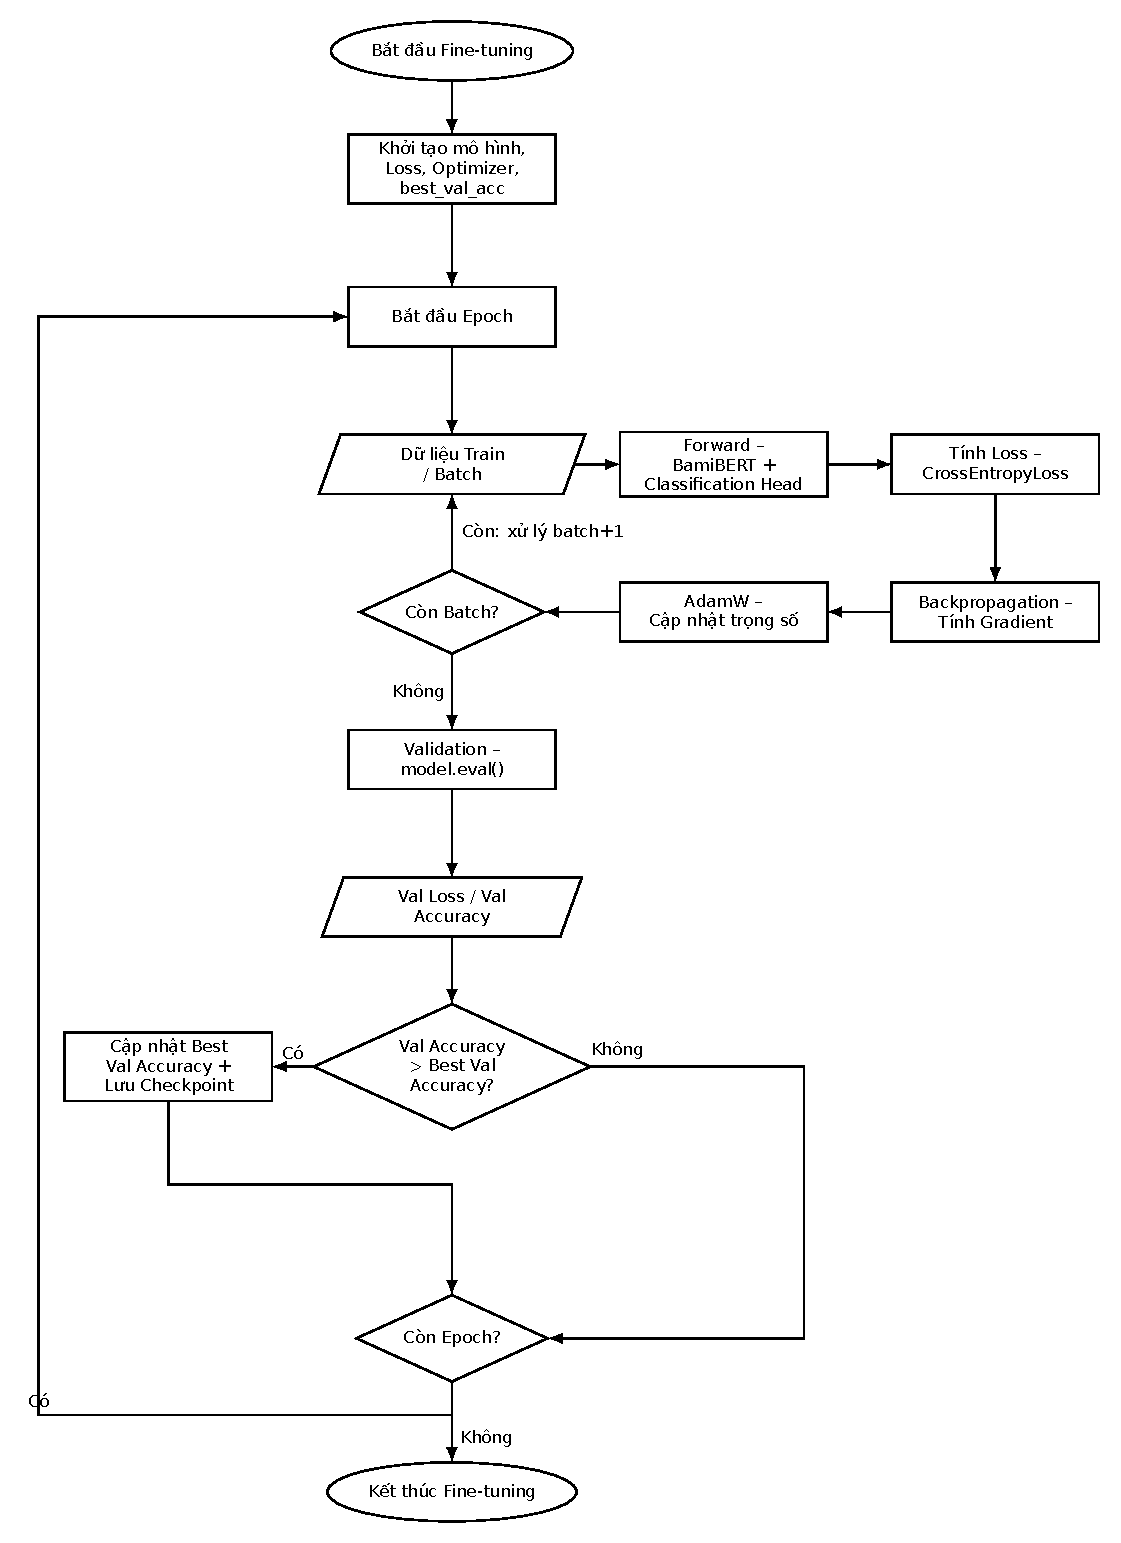
\includegraphics[width=1.1\textwidth]{figures/chapter_03/fine_tune_workflow.pdf}
    \caption{Quá trình fine-tuning}
    \label{fig:fine_tune_workflow}
\end{figure}

\noindent
Qua quá trình fine-tune, mô hình có trọng số tốt nhất được lưu tại \texttt{best\_model.pt} nằm ở epoch số 3 với \texttt{val\_acc = 0.9604}:

\begin{figure}[H]
    \centering
    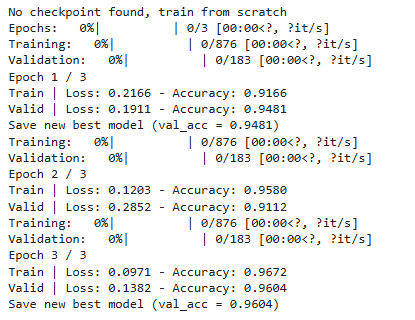
\includegraphics[width=0.5\textwidth]{images/chapter_03/img_24.png}
    \caption{Điểm của mô hình huấn luyện qua các epoch}
    \label{fig:nlp}
\end{figure}

\section{Xây dựng chức năng giải thích}
\subsection{Tổng quan quy trình giải thích}
Sau khi mô hình đã đưa ra dự đoán, hệ thống còn kết hợp chức năng giải thích, giải thích ở đây là gồm hai loại, đó là giải thích mức độ đóng góp của từng token dựa trên kết quả dự đoạn và giải
thích dựa trên các chỉ số định lượng, các token đó bằng ngôn ngữ tự nhiên thông qua mô hình LLM.

\vspace{\baselineskip}
\noindent
Quy trình cụ thể như sau: Văn bản đầu vào sẽ được chia thành hai luồng, một luồng là sẽ đưa vào mô hình BamiBERT để xử lý đưa ra kết quả dự đoán (1) và luồng còn lại sẽ tính đặc trưng thống kê (2). Luồng (1) sau khi đã 
đưa ra kết quả dự đoán thì sẽ sử dụng thuật toán Integrated Gradients (XAI) để bắt đầu tính attribution scores đối với lại từng token, sau đó nếu người dùng yêu cầu giải thích bằng LLM thì sẽ trích ra các top tokens có score
cao nhất còn không thì sẽ hiển thị kết quả dưới dạng highlight. Luồng (2) sẽ thực hiện tính các đặc trưng thống kê, các đặc trưng ở đây cụ thể là mật độ dấu câu, độ dài câu, số câu,\dots làm các giá trị định lượng cho LLM. Sau
đó kết quả từ hai luồng sẽ được tổng hợp lại và sẽ đưa vào LLM (Gemini) để sinh ra giải thích. 

\vspace{\baselineskip}
\noindent
Luồng hoạt động được thể hiện bằng sơ đồ sau:

\begin{figure}[H]
    \centering
    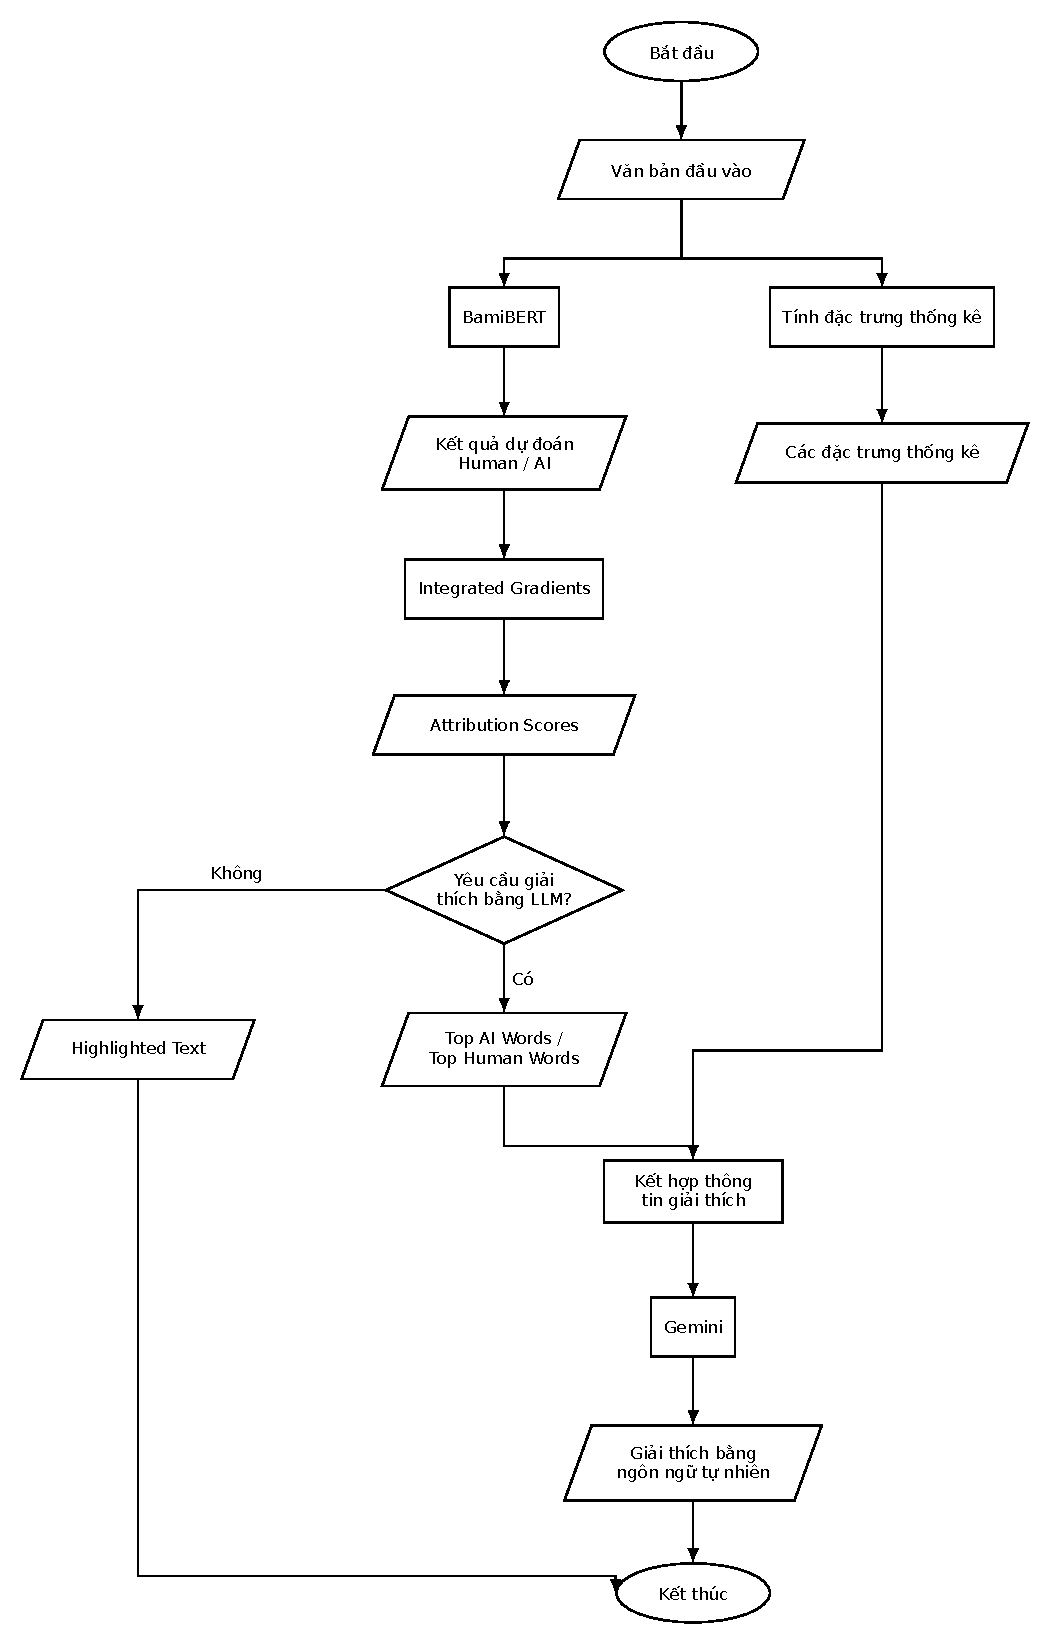
\includegraphics[width=1.0\textwidth]{figures/chapter_03/explain_workflow.pdf}
    \caption{Quá trình đưa ra giải thích}
    \label{fig:fine_tune_workflow}
\end{figure}

\subsection{Tính toán mức độ đóng góp bằng Integrated Gradients}
Trong hệ thống, mức độ đóng góp của từng token sẽ được tính bằng thuật toán Integrated Gradients, thông qua lớp \texttt{LayerIntegratedGradients} của module \texttt{captum}.

\begin{lstlisting}[style=pythoncode]
self.lig = LayerIntegratedGradients(self._forward_func, self.model.bert.embeddings)

def _forward_func(self, input_ids, attention_mask):
    logits = self.model(input_ids, attention_mask)
    return logits
\end{lstlisting}
\captionof{listing}{Khởi tạo \texttt{LayerIntegratedGradients}}

Lớp \texttt{LayerIntegratedGradients} sẽ tính toán mức độ attribution của từng token đầu vào. Trong đó, lớp embedding của mô hình BamiBERT được chọn làm lớp mục tiêu để tính attribution, vì 
lớp này là lớp biểu diễn vector của từng token, do đó attribution sẽ được tính tại lớp này và quy về từng token rồi ánh xạ ngược lại từng từ/cụm từ trong văn bản. Hàm lan truyển sẽ nhận \texttt{input\_ids} và
\texttt{attention\_mask} làm đầu vào để tính giá trị logits, làm đầu ra tương ứng cho các lớp cần phân loại.

\begin{lstlisting}[style=pythoncode]
encoding = self.tokenizer(
        text, max_length=self.max_length, truncation=True,
        padding='max_length', return_tensors='pt',
        return_offsets_mapping=True # return position of each token
        )
input_ids = encoding['input_ids'].to(self.device)
attention_mask = encoding['attention_mask'].to(self.device)
offsets = encoding['offset_mapping'][0].tolist()  # [(start,end), ...] from original text

baseline_ids = torch.full_like(input_ids, self.tokenizer.pad_token_id)
\end{lstlisting}
\captionof{listing}{Chuẩn bị đầu vào và baseline cho quá trình tính attribution}

Trước khi tính attribution thì văn bản đầu vào sẽ được chuyển đổi thành \texttt{input\_ids} và \texttt{attention\_mask} thông qua tokenizer của BamiBERT. Ngoài ra hệ thống còn lưu lại vị trí
của từng token trên văn bản gốc thông qua \texttt{offset\_mapping}, ví dụ như chuỗi sau: "Tôi thích AI" sẽ được ánh xạ thành các chuỗi chỉ số "01234...." thì token "Tôi" sẽ được ánh xạ thành (0, 2). Việc
lưu lại vị trí nhằm hỗ trợ cho bước quy đổi giá trị attribution về từ hoặc cụm từ sau này. \texttt{baseline\_ids} đơn giản là làm đầu vào tham chiếu, tức là tạo một chuỗi có cùng kích thước với \texttt{input\_ids},
trong đó các token được thay bằng token \texttt{<PAD>} làm điểm xuất phát để IG đánh giá mức độ thay đổi khi chuyển từ baseline sang văn bản thực tế. Từ sự thay đổi đó, mức độ đóng góp của từng token qua kết quả dự
đoán được xác định.

\begin{lstlisting}[style=pythoncode]
attributions, delta = self.lig.attribute(
        inputs=input_ids, baselines=baseline_ids,
        additional_forward_args=(attention_mask,),
        target=target_label, return_convergence_delta=True, n_steps=n_steps
    )
\end{lstlisting}
\captionof{listing}{Thực hiện tính attribution}
Sau bước chuẩn bị đầu vào và baseline, attribution sẽ được tính thông qua hàm \texttt{attribute} của lớp \texttt{LayerIntegratedGradients} riêng cho lớp mục tiêu \texttt{target\_label}. Đồng thời còn để biết từ baseline đến
văn bản thật thì output của mô hình đã thay đổi bao nhiêu thì phải thông qua tham số định nghĩa số bước nội suy (\texttt{n\_steps}). Bên cạnh đó, tham số \texttt{return\_convergence\_delta} được sử dụng để đánh giá mức độ hội tụ
hay là độ chính xác của thuật toán IG, tức là giá trị này sẽ tính được sai số lệch giữa tổng attribution tính được so với mức thay đổi đầu ra thực tế giữa mô hình đầu vào so với baseline.

\subsection{Xử lý và tổng hợp Attribution}
Sau khi đã có attribution, giá trị của nó vẫn được biểu diễn theo vector embedding nhiều chiều, cụ thể là 768 chiều. Do đó, ta cần một bước để tổng hợp các giá trị attribution trên toàn bộ chiều của vector embedding thành một giá trị 
đại diện cho mức độ đóng góp của từng token.

\begin{lstlisting}[style=pythoncode]
attributions = attributions.sum(dim=-1).squeeze(0)
attributions = attributions / (torch.norm(attributions) + 1e-10) # keep in stable range
syllable_scores = attributions.cpu().detach().numpy()
\end{lstlisting}
\captionof{listing}{Tổng hợp và chuẩn hóa giá trị attribution}

Ở đây, ta sẽ tính tổng hợp bằng cách tính tổng toàn bộ các attribution trên vector nhiều chiều thống qua \texttt{attribution.sum(dim=-1)}, sau đó ta sẽ chuẩn hóa giá trị vừa tính được về cùng một thang đo để thuận tiện cho việc so sánh và
trực quan hóa.

\begin{lstlisting}[style=pythoncode]
attributions = attributions.sum(dim=-1).squeeze(0)
attributions = attributions / (torch.norm(attributions) + 1e-10) # keep in stable range
syllable_scores = attributions.cpu().detach().numpy()
\end{lstlisting}
\captionof{listing}{Tổng hợp và chuẩn hóa giá trị attribution}

Sau khi đã chuẩn hóa xong, các attribution lúc này vẫn là một giá trị của từng token nên ta phải thực hiện bước ánh xạ sang attribution của từng từ hay cụm từ.
\begin{lstlisting}[style=pythoncode]
from underthesea import word_tokenize as vn_word_tokenize

    vn_words = vn_word_tokenize(text)  # for example: ['Samsung', 'đang', 'gặp', 'khó khăn', ...]

# Step 3: Map for each compound nouns -> positional range from original text
word_spans = []
cursor = 0
for w in vn_words:
    start = text.find(w, cursor)
    if start == -1: # unnecessary, defensive programming
            continue
        end = start + len(w)
        word_spans.append((w, start, end))
        cursor = end

    # Step 4: Combine attribution of syllable-tokens to fall in range of each compound nouns
    word_results = []
    for word, w_start, w_end in word_spans:
        scores_in_span = [
            syllable_scores[i] for i, (s, e) in enumerate(offsets)
            if s < w_end and e > w_start and not (s == 0 and e == 0)  # drop special tokens
        ]
        if scores_in_span:
            word_results.append((word, float(np.mean(scores_in_span))))
\end{lstlisting}
\captionof{listing}{Ánh xạ giá trị token sang từ/cụm từ}
Ở đây, ta sẽ sử dụng hàm \texttt{word\_tokenize} của module \texttt{underthesea} để tách chuỗi văn bản thành các token tiếng Việt tương ứng, từ đơn
tách thành từ đơn cũng như từ ghép tách thành từ ghép, sau đó thực hiện gom attribution của các token có phần ký tự giao với từ hay cụm từ đang xét 
(\texttt{syllable\_scores[i] for i, (s, e) in enumerate(offsets)}). Nếu như gặp từ ghép thì ta sẽ tính trung bình các attribution của các token trong từ đó.

\subsection{Sinh giải thích bằng LLM}
Bênh cạnh khả năng giải thích dựa trên attribution score của từng từ thì hệ thống còn xây dựng thêm chức năng giải thích bằng ngôn ngữ tự nhiên. Đầu tiên, để cho lời
nhắc (prompt) mà sát với các kết quả mà hệ thống đưa ra thì ta cần phải tính thêm các giá trị định lượng và lọc ra các từ, cụm từ mà có attribution score cao để đưa vào 
mô hình LLM giải thích.

\begin{lstlisting}[style=pythoncode]
def compute_signals(cleaned_text, tokens, scores, top_k = 8):
    paired = sorted(zip(tokens, scores), key=lambda x: abs(x[1]), reverse=True)
    top_ai_words = [w for w, s in paired if s > 0][:top_k]
    top_human_words = [w for w, s in paired if s < 0][:top_k]

    sentences = [s.strip() for s in re.split(r'[.!?]', cleaned_text) if s.strip()]
    sentence_lengths = [len(s.split()) for s in sentences]
    punct_count = len(re.findall(r'[^\w\sÀ-ỹ]', cleaned_text))

    return {
        'top_ai_words': top_ai_words,
        'top_human_words': top_human_words,
        'sentence_count': len(sentences),
        'avg_sentence_length': sum(sentence_lengths) / max(len(sentence_lengths), 1),
        'sentence_length_std': statistics.pstdev(sentence_lengths) if len(sentence_lengths) > 1 else 0.0,
        'punctuation_density': punct_count / max(len(cleaned_text), 1)
    }
\end{lstlisting}
\captionof{listing}{Lọc các token có attribution lớn nhất và tính các giá trị định lượng}

\begin{table}[H]
\centering
\caption{Ý nghĩa các giá trị được tính trong quá trình sinh giải thích bằng LLM}
\label{tab:attribution-signals}
\begin{tabular}{|p{0.32\textwidth}|p{0.58\textwidth}|}
\hline
\textbf{Giá trị} & \textbf{Ý nghĩa} \\
\hline
\texttt{top\_ai\_words} & Các từ/cụm từ có mức độ đóng góp mạnh theo hướng nhãn AI \\
\hline
\texttt{top\_human\_words} & Các từ/cụm từ có mức độ đóng góp mạnh theo hướng nhãn Human \\
\hline
\texttt{sentence\_count} & Số lượng câu trong văn bản, phản ánh quy mô cấu trúc câu của văn bản \\
\hline
\texttt{avg\_sentence\_length} & Độ dài câu trung bình, cho biết một văn bản đó có xu hướng câu ngắn hay dài \\
\hline
\texttt{sentence\_length\_std} & Độ lệch chuẩn của câu, cho biết mức độ biến thiên của câu trong văn bản, tức là các câu trong văn bản có độ dài đồng đều hay không \\
\hline
\texttt{punctuation\_density} & Mật độ dấu câu, phản ánh mức độ dấu câu hay kí tự đặc biệt của văn bản \\
\hline
\end{tabular}
\end{table}

\section{Xây dựng backend}
\subsection{Mô hình thực thể kết hợp (ERD)}

\begin{figure}[H]
    \centering
    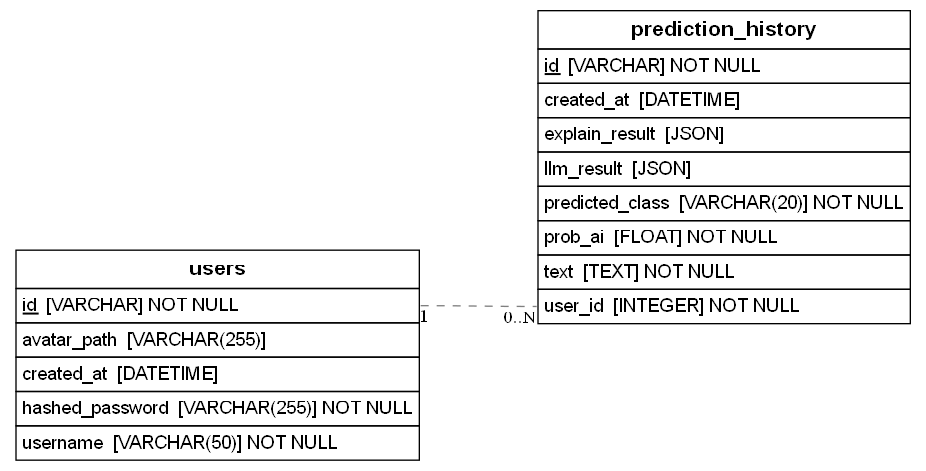
\includegraphics[width=0.8\textwidth]{images/chapter_03/img_25.png}
    \caption{Lược đồ trực quan hóa CSDL}
    \label{fig:fine_tune_workflow}
\end{figure}

\subsection{Thiết kế chi tiết các bảng}
\subsubsection{Bảng user}
Bảng này lưu trữ thông tin cho từng tài khoản người dùng.

\begin{table}[H]
\centering
\caption{Cấu trúc bảng \texttt{users}}
\label{tab:users-schema}
\begin{tabular}{|p{0.24\textwidth}|p{0.20\textwidth}|p{0.46\textwidth}|}
\hline
\textbf{Tên cột} & \textbf{Kiểu dữ liệu} & \textbf{Mô tả} \\
\hline
\texttt{id} & \texttt{VARCHAR(40)} & Khóa chính, định danh duy nhất của người dùng. \\
\hline
\texttt{username} & \texttt{VARCHAR(50)} & Tên đăng nhập duy nhất của người dùng. \\
\hline
\texttt{hashed\_password} & \texttt{VARCHAR(255)} & Mật khẩu đã được băm, dùng để xác thực người dùng. \\
\hline
\texttt{avatar\_path} & \texttt{VARCHAR(255)} & Đường dẫn đến ảnh đại diện; có thể để trống. \\
\hline
\texttt{created\_at} & \texttt{DATETIME} & Thời điểm tài khoản được tạo, mặc định là thời gian hiện tại. \\
\hline
\end{tabular}
\end{table}

\subsubsection{Bảng prediction history}
Bảng này lưu trữ đoạn văn bản và kết quả dự đoán mà người dùng đã từng sử dụng.

\begin{table}[H]
\centering
\caption{Cấu trúc bảng \texttt{prediction\_history}}
\label{tab:prediction-history-schema}
\begin{tabular}{|p{0.24\textwidth}|p{0.20\textwidth}|p{0.46\textwidth}|}
\hline
\textbf{Tên cột} & \textbf{Kiểu dữ liệu} & \textbf{Mô tả} \\
\hline
\texttt{id} & \texttt{VARCHAR(40)} & Khóa chính, định danh duy nhất của bản ghi dự đoán. \\
\hline
\texttt{user\_id} & \texttt{VARCHAR(40)} & Khóa ngoại tham chiếu đến \texttt{users.id}, xác định người thực hiện dự đoán. \\
\hline
\texttt{text} & \texttt{TEXT} & Đoạn văn bản được đưa vào hệ thống để phân loại. \\
\hline
\texttt{predicted\_class} & \texttt{VARCHAR(20)} & Nhãn dự đoán của mô hình, chẳng hạn AI hoặc Human. \\
\hline
\texttt{prob\_ai} & \texttt{FLOAT} & Xác suất văn bản được dự đoán là do AI tạo ra. \\
\hline
\texttt{explain\_result} & \texttt{JSON} & Kết quả giải thích dựa trên attribution score; có thể để trống. \\
\hline
\texttt{llm\_result} & \texttt{JSON} & Kết quả giải thích được sinh bởi mô hình ngôn ngữ lớn; có thể để trống. \\
\hline
\texttt{created\_at} & \texttt{DATETIME} & Thời điểm bản ghi dự đoán được tạo, mặc định là thời gian hiện tại. \\
\hline
\end{tabular}
\end{table}

\subsection{Thiết kế các API chính cho hệ thống}
Trong hệ thống, các API chính bao gồm: API dự đoán (\texttt{/predict}), API giải thích theo highlight text (\texttt{/explain}) và API giải thích
bằng LLM (\texttt{/explain-llm}).

\begin{table}[H]
    \centering
    \caption{Các API chính của hệ thống}
    \label{tab:main-apis}
    \begin{tabular}{|p{0.30\textwidth}|p{0.60\textwidth}|}
        \hline
        \textbf{API chính} & \textbf{Ý nghĩa} \\
        \hline
        \texttt{POST /predict} & Nhận văn bản đầu vào, thực hiện phân loại văn bản là do AI tạo ra hay do con người viết, đồng thời lưu kết quả dự đoán vào lịch sử nếu người dùng đã đăng nhập. \\
        \hline
        \texttt{POST /explain} & Phân tích mức độ đóng góp của từng token trong văn bản bằng Integrated Gradients và trả về kết quả để giao diện highlight các từ. \\
        \hline
        \texttt{POST /explain-llm} & Kết hợp kết quả dự đoán, attribution và các đặc trưng của văn bản để tạo lời giải thích bằng ngôn ngữ tự nhiên thông qua mô hình LLM. \\
        \hline
    \end{tabular}
\end{table}

\section{Xây dựng giao diện}
Hệ thống được xây dựng bằng ReactJS, gồm các chức năng sau:
\subsection{Giao diện đăng ký}
\begin{figure}[H]
    \centering
    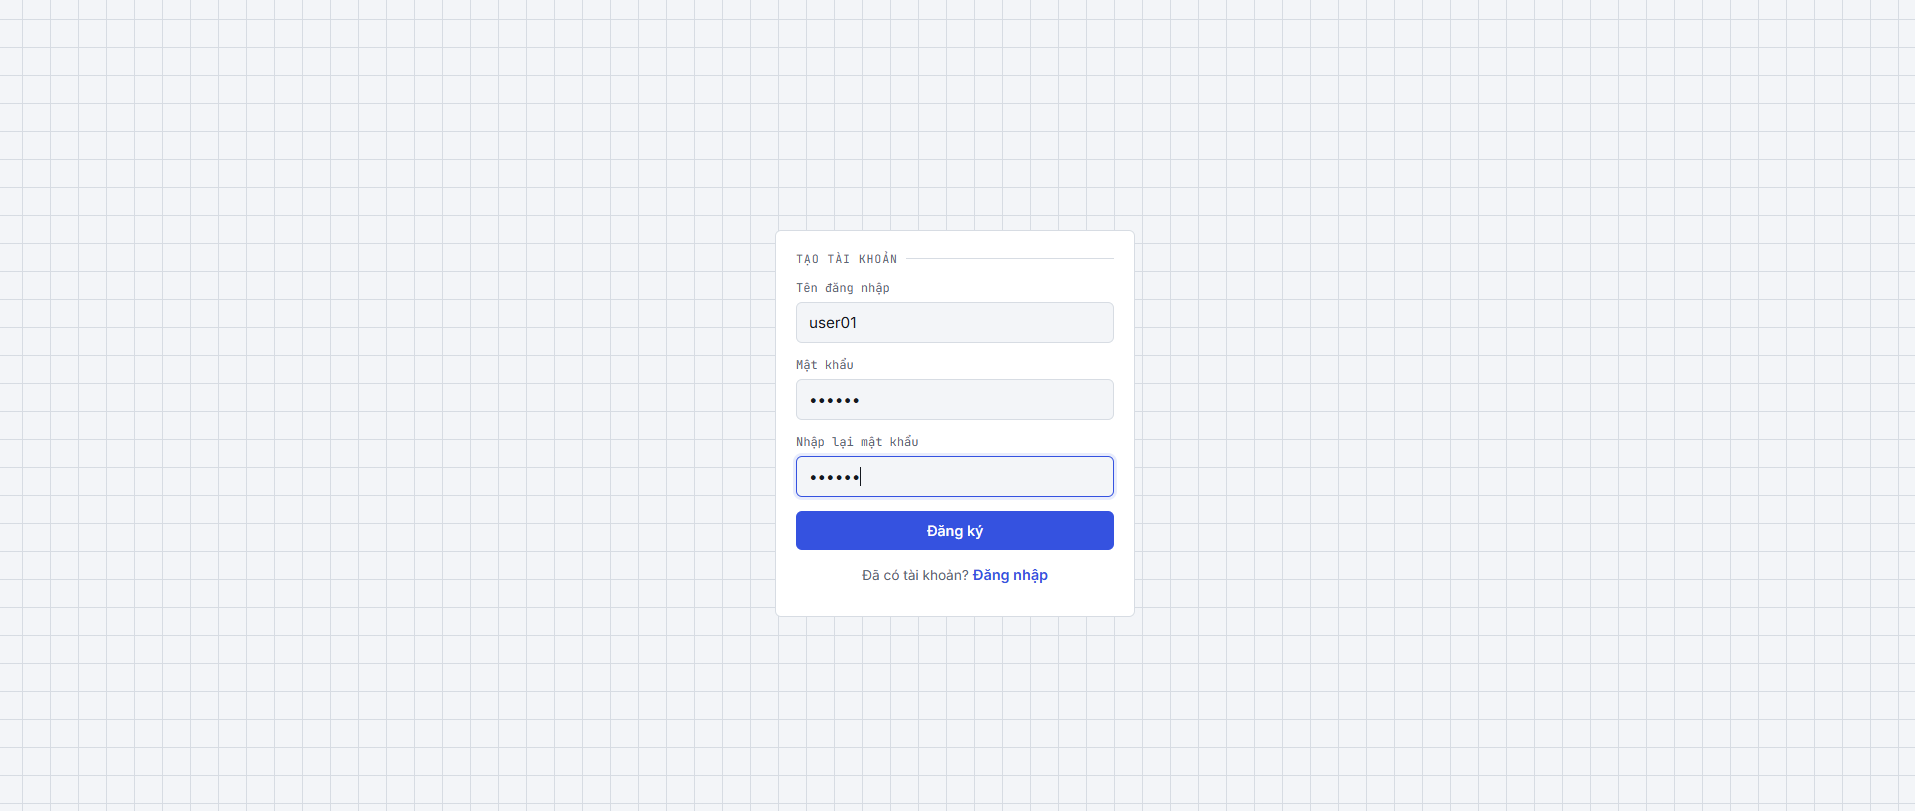
\includegraphics[width=1.0\textwidth]{images/chapter_03/img_26.png}
    \caption{Giao diện đăng ký tài khoản}
    \label{fig:nlp}
\end{figure}

\subsection{Giao diện đăng nhập}
\begin{figure}[H]
    \centering
    
\includegraphics[width=1.0\textwidth]{images/chapter_03/img_27.png}
    \caption{Giao diện đăng nhập tài khoản}
    \label{fig:nlp}
\end{figure}

\subsection{Giao diện trang chủ}
\begin{figure}[H]
    \centering
    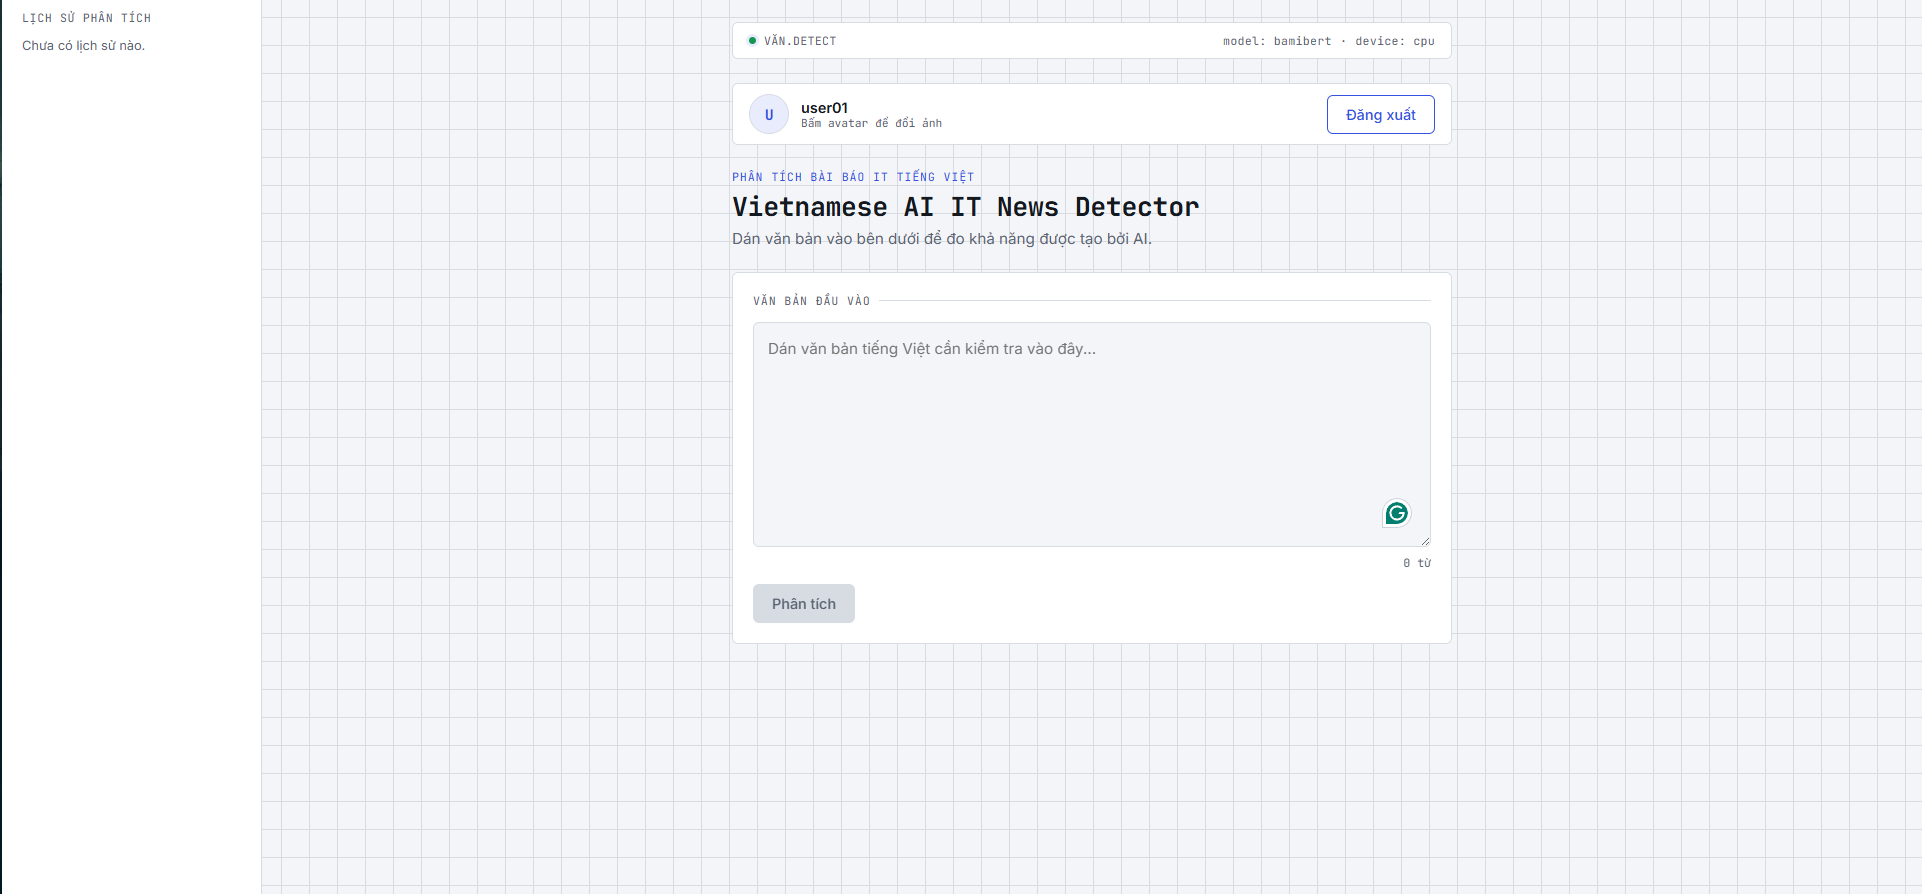
\includegraphics[width=1.0\textwidth]{images/chapter_03/img_28.png}
    \caption{Giao diện trang chủ}
    \label{fig:nlp}
\end{figure}

\subsection{Giao diện dự đoán}
\begin{figure}[H]
    \centering
    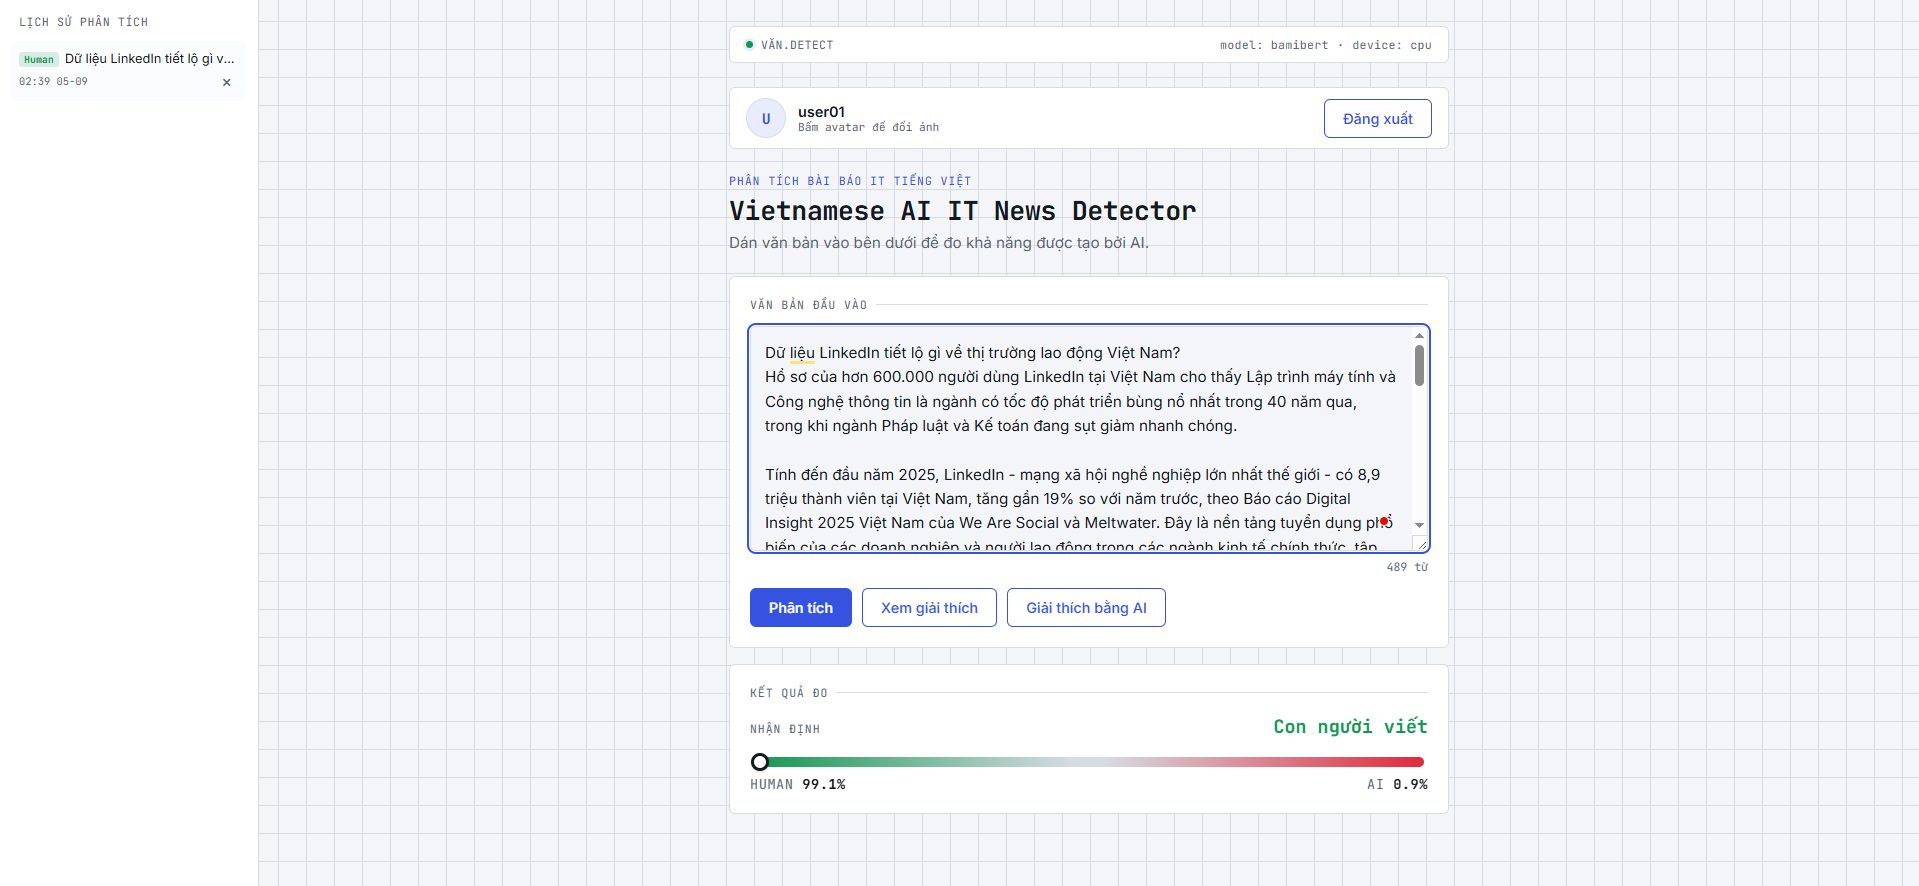
\includegraphics[width=1.0\textwidth]{images/chapter_03/img_29.png}
    \caption{Giao diện dự đoán}
    \label{fig:nlp}
\end{figure}

\subsection{Giao diện lịch sử}
\begin{figure}[H]
    \centering
    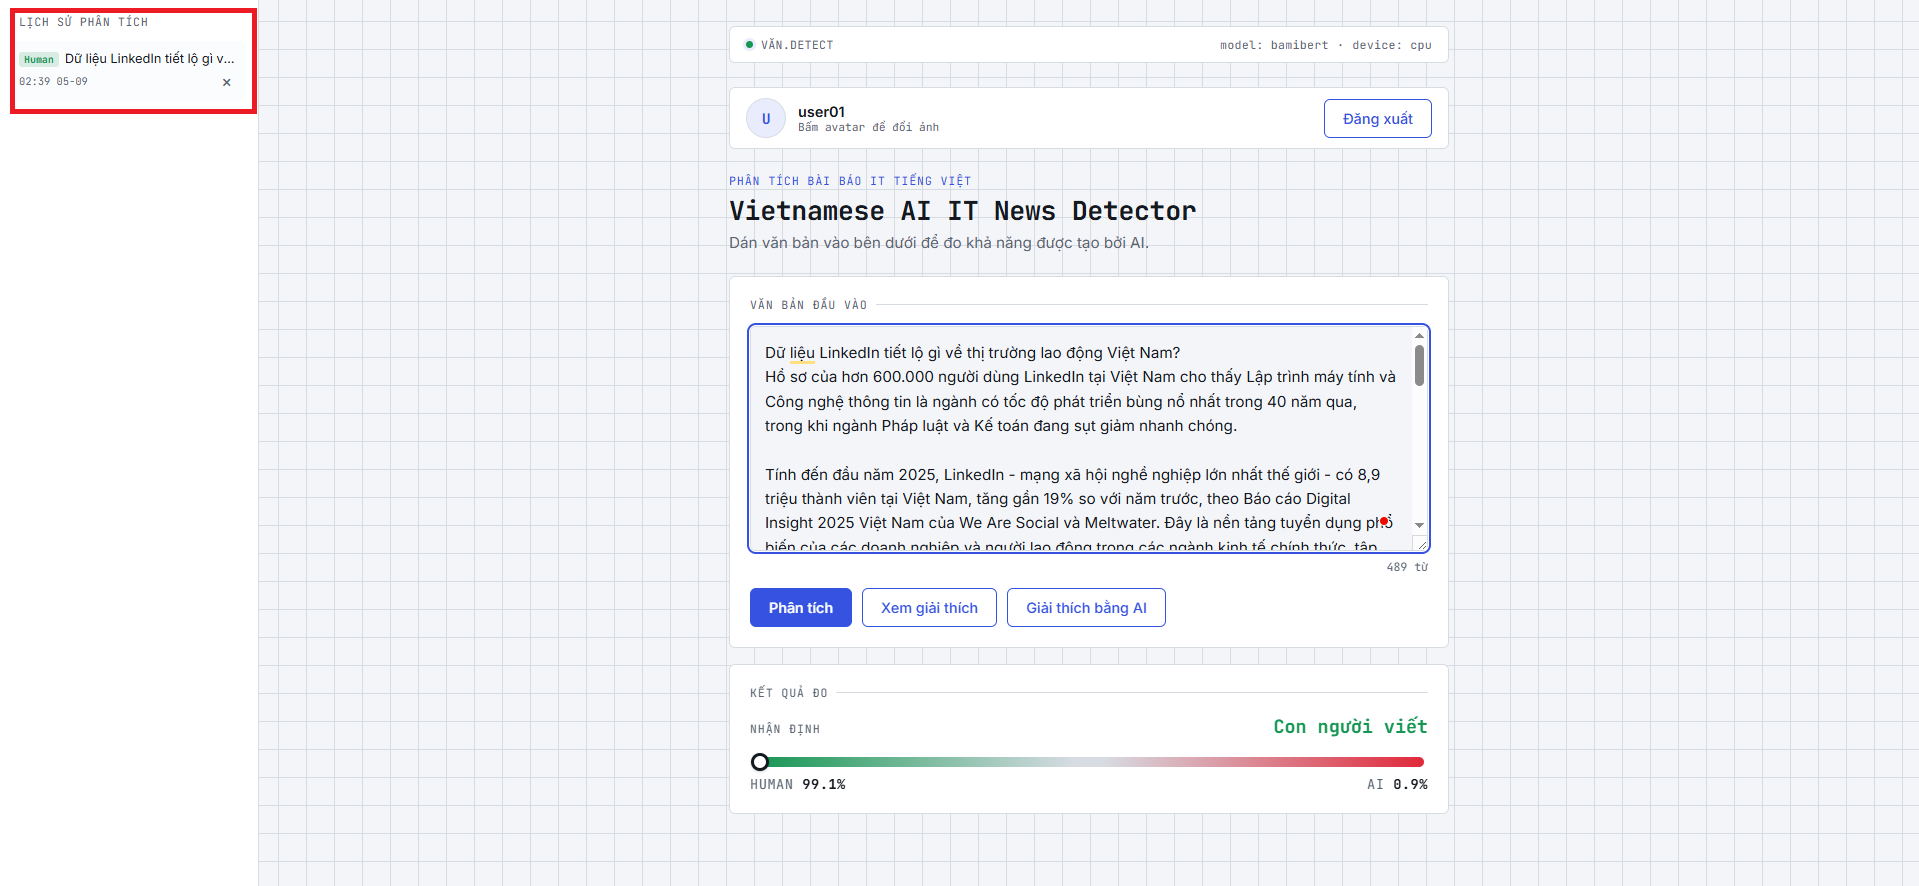
\includegraphics[width=1.0\textwidth]{images/chapter_03/img_30.png}
    \caption{Giao diện hiển thị lịch sử}
    \label{fig:nlp}
\end{figure}

\subsection{Giao diện giải thích highlight text}
\begin{figure}[H]
    \centering
    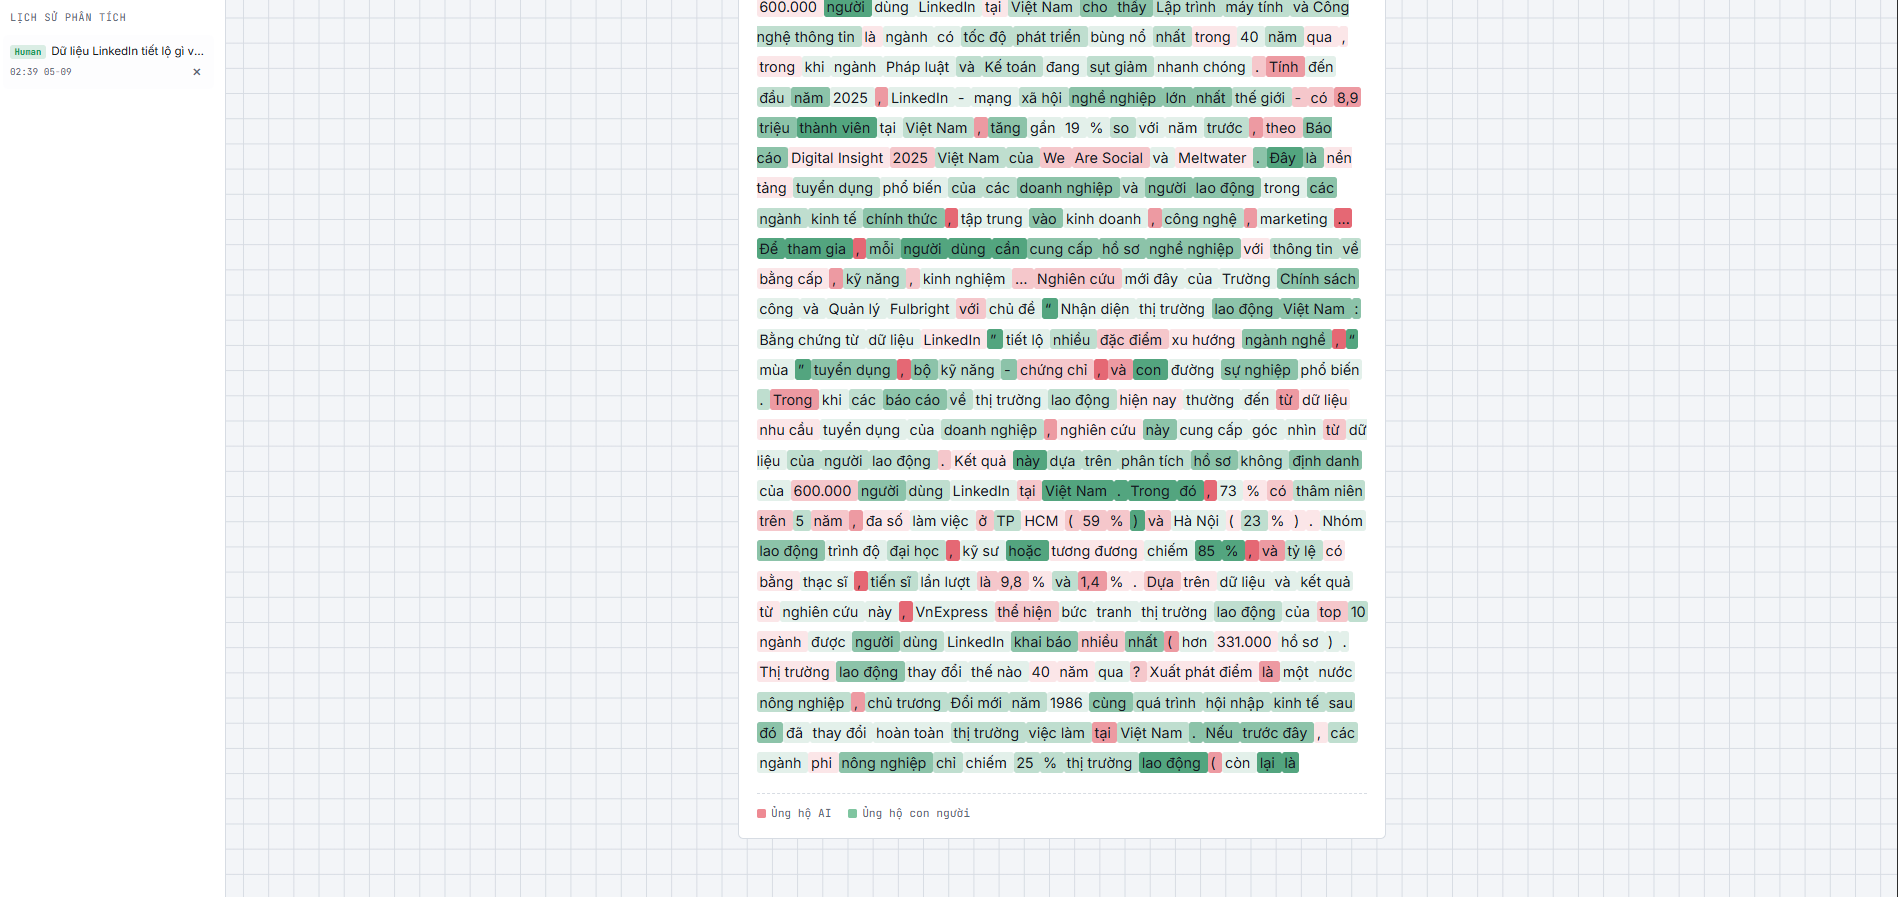
\includegraphics[width=1.0\textwidth]{images/chapter_03/img_31.png}
    \caption{Giao diện hiển thị text highlight}
    \label{fig:nlp}
\end{figure}

\subsection{Giao diện giải thích bằng LLM}
\begin{figure}[H]
    \centering
    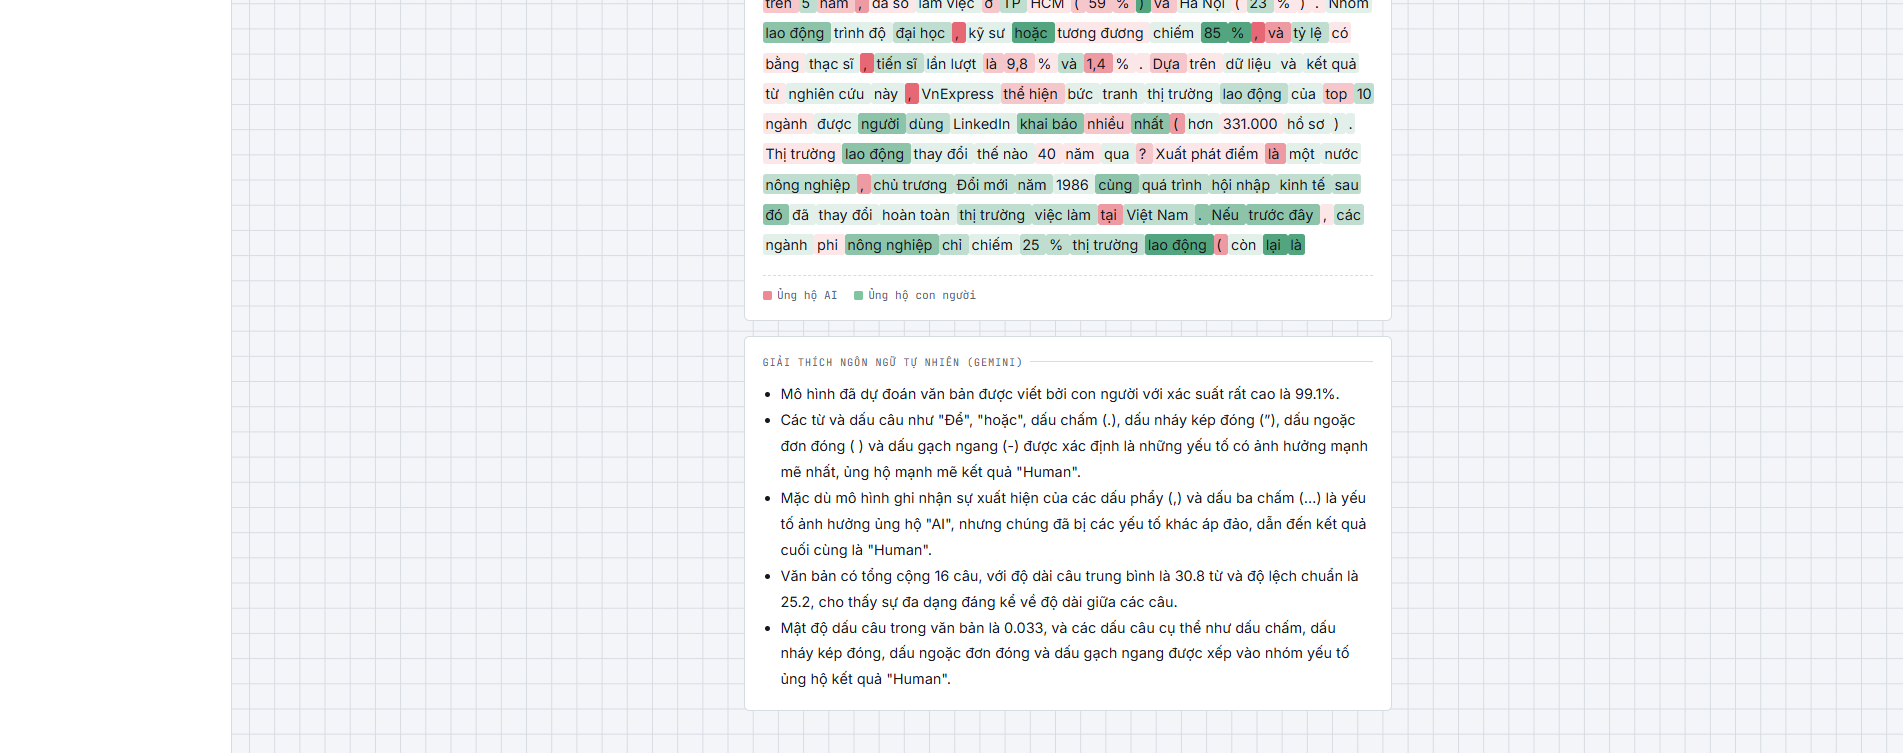
\includegraphics[width=1.0\textwidth]{images/chapter_03/img_32.png}
    \caption{Giao diện hiển thị kết quả giải thích LLM}
    \label{fig:nlp}
\end{figure}
% !TEX root = main.tex
\chapter{Thực nghiệm và đánh giá hệ thống}

\section{Thực nghiệm và đánh giá mô hình phân loại}
\subsection{Các tiêu chí đánh giá}
Để đánh giá mô hình dự đoán, hệ thống sẽ sử dụng tập dữ liệu test đã được tạo ra từ trước (766 mẫu). Các tiêu chí đánh giá bao gồm 4 thành phần sau:
\subsubsection{Độ chính xác (Precision)}
Precision là tỉ lệ số mẫu dương thực tế (Positive) so với tổng số mẫu mà mô hình dự đoán là dương, cho biết mô hình dự đoán một kết quả là "đúng" với độ tin cậy
là bao nhiêu.
\begin{equation}
	\mathrm{Precision} = \frac{TP}{TP + FP}
\end{equation}
Trong đó, $TP$ là số mẫu dương được dự đoán đúng và $FP$ là số mẫu âm bị dự đoán nhầm thành dương.

\subsubsection{Độ bao phủ (Recall)}
Độ bao phủ là tỉ lệ mà mô hình dự đoán là dương tính so với các mẫu vốn dĩ, chắc chắn là dương, cho biết mô hình bỏ sót bao nhiêu mẫu thực tế cần tìm
\begin{equation}
	\mathrm{Recall} = \frac{TP}{TP + FN}
\end{equation}
Trong đó, $FN$ là số mẫu dương bị dự đoán nhầm thành âm.

\subsubsection{Điểm F1 (F1-score)}
F1-score là trung bình điều hòa của Precision và Recall, giúp đánh giá cân bằng giữa độ chính xác và độ bao phủ khi dữ liệu bị mất cân bằng.
\begin{equation}
	\mathrm{F1\text{-}score} = 2 \times \frac{\mathrm{Precision} \times \mathrm{Recall}}{\mathrm{Precision} + \mathrm{Recall}}
\end{equation}

\subsubsection{Đường cong ROC (ROC Curve)}
ROC Curve là một đồ thị biểu diễn khả năng phân loại của mô hình tại các ngưỡng (threshold) khác nhau.

\subsection{Kết quả thực nghiệm}
\subsubsection{Bảng kết quả}
\begin{figure}[H]
    \centering
    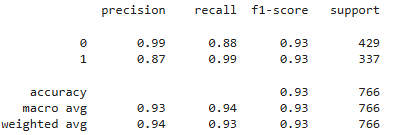
\includegraphics[width=0.6\textwidth]{images/chapter_04/img_33.png}
    \caption{Bảng kết quả thống kê}
    \label{fig:nlp}
\end{figure}

\noindent
Ta có thể thấy mô hình đạt độ chính xác lên tới 93\% và F1-score của hai lớp đều như nhau cũng với 93\%. Ngoài ra, precision rất cao đối với lớp Human và recall
cao đối với AI, cho thấy mô hình dự đoán các văn bản thuộc AI rất tốt nhưng recall của Human hơi thấp hơn (88\%), cho thấy các văn bản Human vẫn bị dự đoán nhầm thành AI.

\subsubsection{Ma trận sai lầm}
\begin{figure}[H]
    \centering
    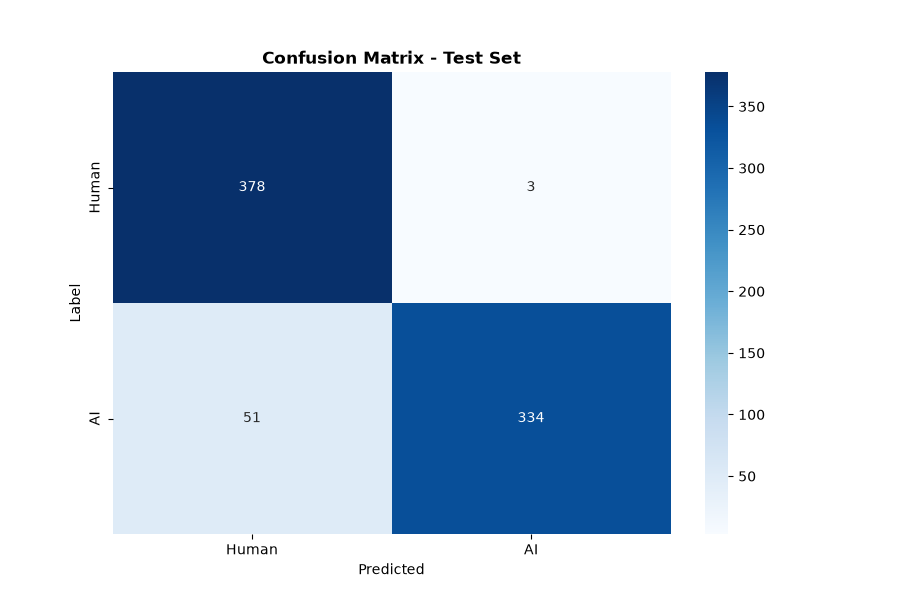
\includegraphics[width=0.8\textwidth]{images/chapter_04/img_34.png}
    \caption{Ma trận sai lầm}
    \label{fig:nlp}
\end{figure}

\noindent
Cụ thể số liệu như sau, qua ma trận nhầm lẫn trên. Ta có thể thấy trong 429 bài báo thì có 378 là dự đoán đúng là Human và 3 bài còn lại dự đoán nhầm là AI. Bên cạnh đó, trong
337 bài thì có 51 bài là AI mà dự đoán nhầm là Human và chỉ dự đoán đúng 334 bài AI còn lại.

\subsubsection{Độ chính xác của ba phương pháp sinh dữ liệu}
\begin{figure}[H]
    \centering
    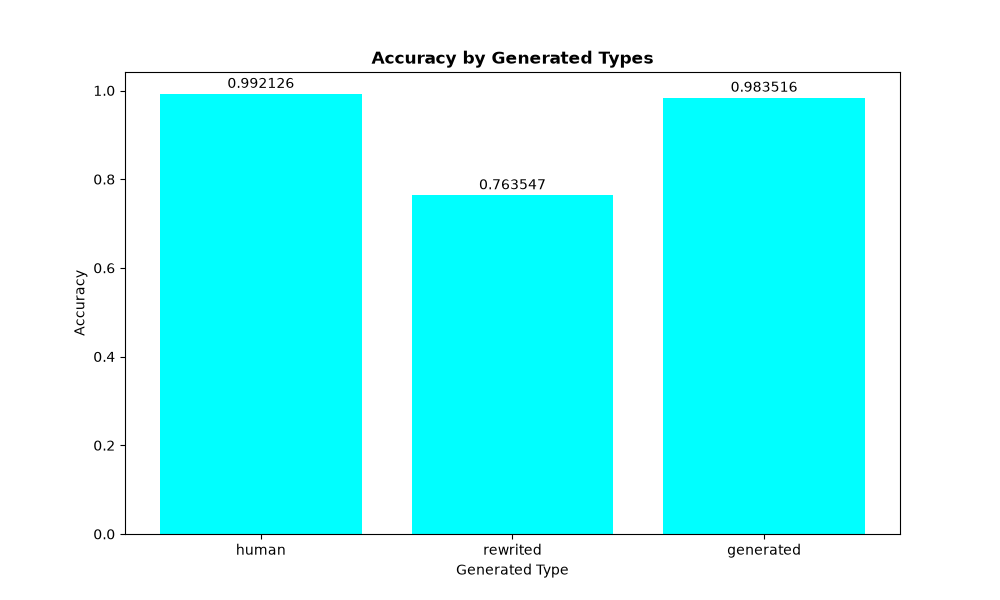
\includegraphics[width=0.9\textwidth]{images/chapter_04/img_35.png}
    \caption{Độ chính xác của ba phương pháp sinh dữ liệu}
    \label{fig:nlp}
\end{figure}

\noindent
Độ chính xác của ba phương pháp tạo dữ liệu như sau: Human: 99\%, AI-Generated: 98\% và AI-Rewrited: 76\%. Điều này cho thấy độ chính xác của mô hình trên tập test tốt nhưng vẫn dự 
đoán sai các văn bản được AI viết lại, độ chính xác thấp hơn hẳn so với hai nhóm còn lại.

\subsubsection{Đường cong ROC}
\begin{figure}[H]
    \centering
    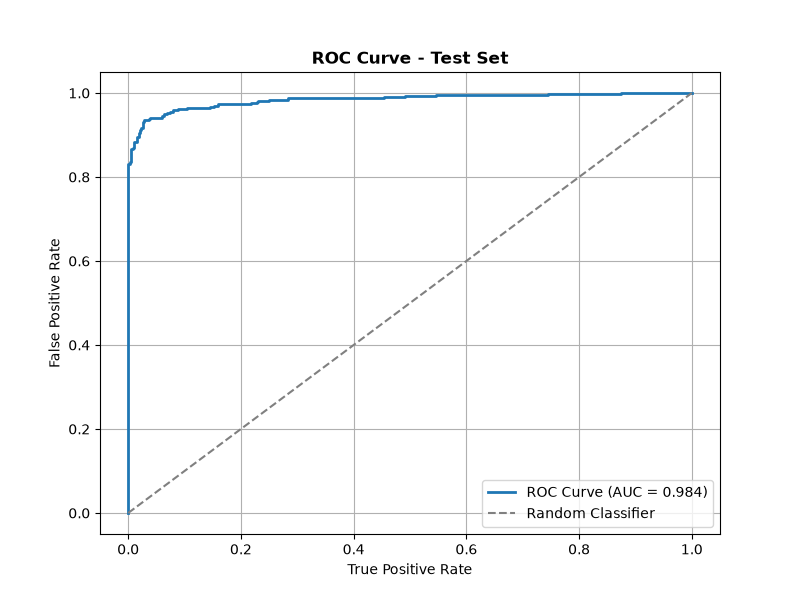
\includegraphics[width=0.8\textwidth]{images/chapter_04/img_36.png}
    \caption{Đường cong ROC}
    \label{fig:nlp}
\end{figure}

\noindent
Đường cong ROC cũng cho thấy mô hình phân biệt tốt hai lớp với độ chính xác rất cao, giá trị AUC lên tới 98\%, là đường cong nằm gần góc trái, mô hình càng dự đoán chính xác thì đường cong càng
gần góc trái hơn, tức là độ bao phủ trên tập dữ liệu lớn hơn.

\section{Đánh giá thuật toán giải thích Integrated Gradients}
\subsection{Đánh giá hội tụ và độ trung thực của giải thích}
\begin{figure}[H]
    \centering
    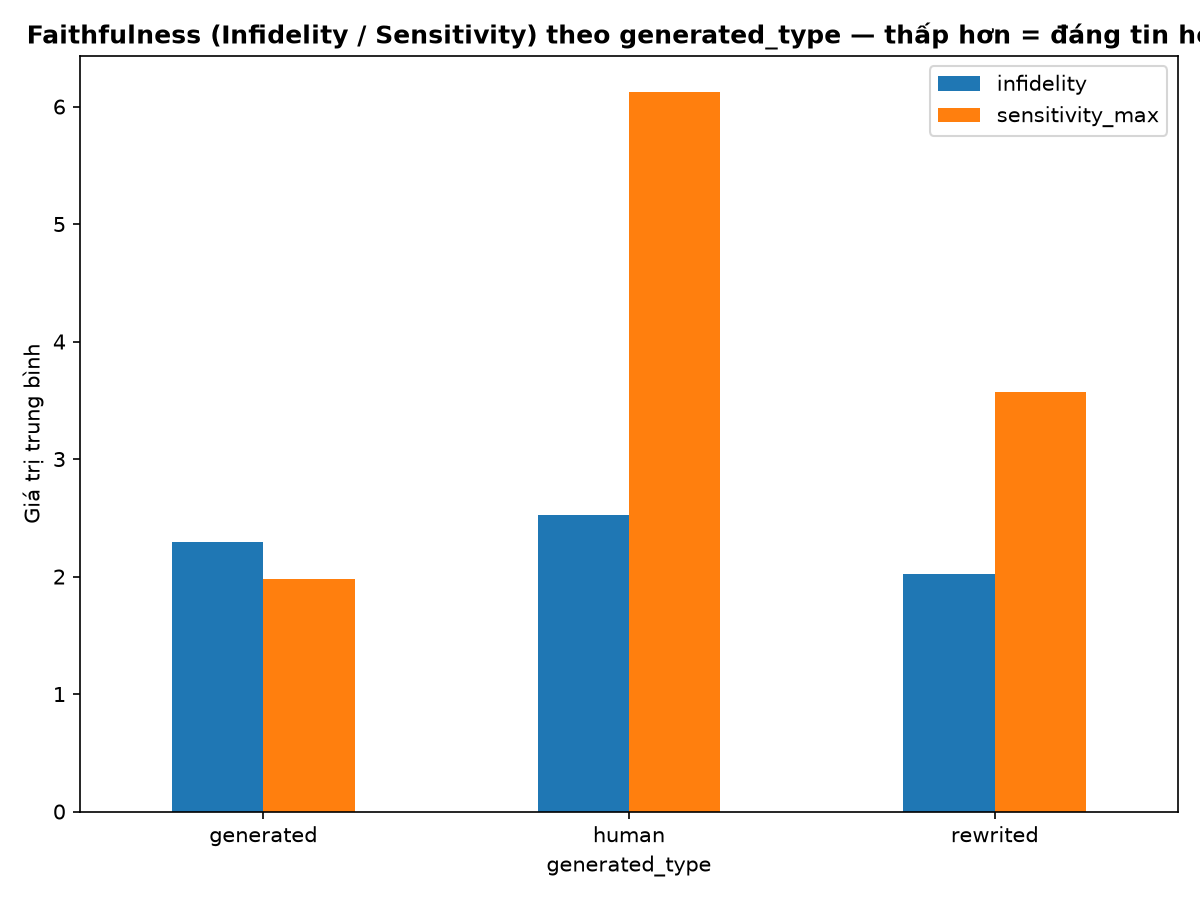
\includegraphics[width=0.8\textwidth]{images/chapter_04/img_37.png}
    \caption{Độ bất trung thực và Độ ổn định}
    \label{fig:nlp}
\end{figure}

\noindent
Độ bất trung thực (Infidelity) sẽ cho biết các điểm attribution có phản ánh đúng mức độ đầu ra của token hay từ đến đầu ra của mô hình hay không, tức là khi ta thay đổi hay bỏ một từ mà điểm attribution cao (từ đó
có mức độ ảnh hưởng lớn đến kết quả) thì đầu ra của mô hình cũng phải thay đổi đáng kể. Infidelity thấp là tốt, vì điều đó cho thấy attribution dự đoán đúng mức độ thay đổi của mô hình khi đầu vào bị thay đổi. Ví dụ, ta xét một chuỗi câu sau: ``I love AI'' và giả sử mô hình trả về xác suất văn bản do AI tạo ra là $0.90$.

\begin{itemize}
    \item \textbf{Trường hợp giải thích tốt:} attribution của token ``AI'' là $+0.70$. Khi thay token này bằng một token trung tính hoặc loại bỏ token, xác suất dự đoán giảm từ $0.90$ xuống $0.35$, tức là thay đổi $0.55$. Mức attribution cao đã phản ánh đúng ảnh hưởng lớn của token ``AI'', nên sai lệch giữa attribution và thay đổi thực tế nhỏ; do đó Infidelity thấp.
    \item \textbf{Trường hợp giải thích kém:} attribution của token ``love'' là $+0.35$. Tuy nhiên, khi thay hoặc loại bỏ token này, xác suất dự đoán chỉ giảm từ $0.90$ xuống $0.89$, tức là thay đổi $0.01$. Mặc dù attribution cho rằng token ``love'' có ảnh hưởng đáng kể, đầu ra của mô hình gần như không thay đổi. Vì vậy, sai lệch lớn và Infidelity cao, cho thấy giải thích không trung thực.
\end{itemize}

Độ nhạy (Sensitivity) cho biết mức độ ổn định của attribution khi đầu vào có sự thay đổi nhẹ, tức là nếu đầu vào có thay đổi một chút thì liệu các attribution score có thay đổi đáng kể hay không. Ví dụ, ta xét một chuỗi sau: "AI đang phát triển mạnh trong lĩnh vực công nghệ."

\begin{itemize}
    \item \textbf{Trường hợp giải thích ổn định:} với câu gốc, attribution của các token ``AI'', ``phát triển'' và ``công nghệ'' lần lượt là $+0.40$, $+0.25$ và $+0.15$. Khi thay token ``mạnh'' bằng ``rất mạnh'', các attribution tương ứng chỉ thay đổi nhẹ, chẳng hạn thành $+0.39$, $+0.26$ và $+0.14$. Vì đầu vào chỉ thay đổi một token nhưng cách mô hình giải thích gần như được giữ nguyên, Sensitivity thấp và đây là kết quả tốt.
    \item \textbf{Trường hợp giải thích không ổn định:} với cùng thay đổi nhỏ ``mạnh'' thành ``rất mạnh'', attribution của các token trên lại thay đổi mạnh, chẳng hạn từ $+0.40$, $+0.25$, $+0.15$ thành $-0.10$, $+0.65$, $+0.02$. Khi đó, một thay đổi nhỏ trong câu đã làm mô hình phân bổ mức độ ảnh hưởng sang các token khác một cách đáng kể. Sensitivity cao, cho thấy attribution thiếu ổn định và giải thích không đáng tin cậy.
\end{itemize}

Qua hình 38, ta có thể thấy giá trị infidelity trung bình của ba nhóm tương đối gần nhau và thấp, dao động từ 2 - 2.5, trong đó nhóm \texttt{rewrited} đạt giá trị thấp nhất. Điều này cho thấy mức độ trung thực của nhóm \texttt{rewrited} tốt hơn so với hai nhóm còn lại. Ngoài ra, đối với sensitivity thì nhóm \texttt{generated} đạt giá trị thấp nhất (xấp xỉ 2.0), cho thấy tính ổn định của nhóm \texttt{generated} tốt hơn so với hai nhóm còn lại nhưng
nhóm Human thì cao nhất (6.0), cho thấy attribution của nhóm này thay đổi đáng kể khi thay đổi nhỏ đầu vào.

\subsection{Phân tích kết quả attribution}
Sau đây là kết quả attribution score của các token tương ứng với bài báo của ba phương pháp tạo dữ liệu:

\begin{figure}[H]
    \centering
    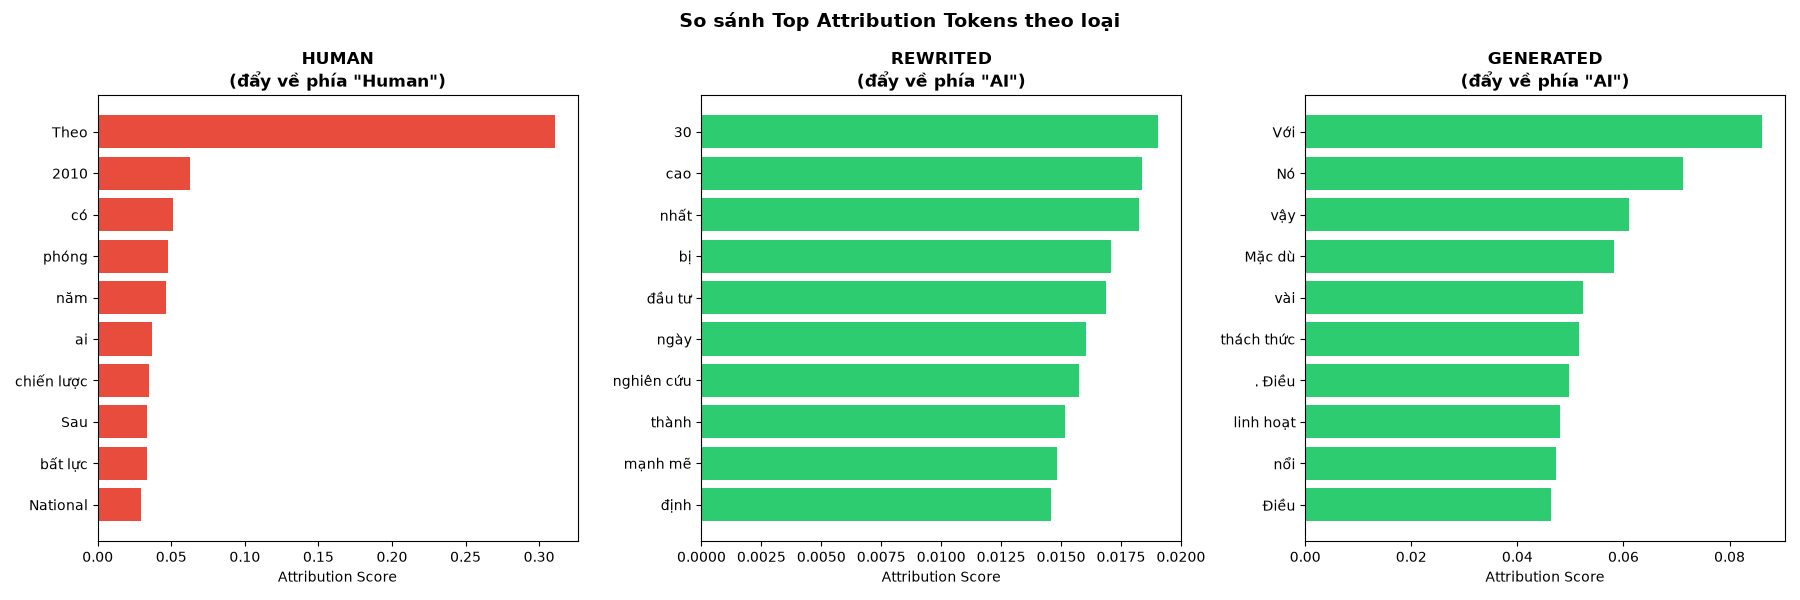
\includegraphics[width=1.0\textwidth]{images/chapter_04/img_38.png}
    \caption{Attribution score của các token tương ứng với ba phương pháp tạo dữ liệu}
    \label{fig:nlp}
\end{figure}

\section{Đánh giá kết quả giải thích bằng LLM}
\subsection{Thiết lập sinh giải thích}
\begin{Verbatim}[fontsize=\small, frame=single, rulecolor=\color{gray!20}, formatcom=\color{black}]
PROMPT_TEMPLATE = """
Bạn là trợ lý giải thích kết quả của một mô hình phát hiện văn bản AI tiếng Việt.
Model đã dự đoán: {predicted_class} (xác suất {pred_prob:.1%}).

Bằng chứng đã tính được (KHÔNG được suy đoán thêm ngoài các số liệu này):
- Từ ảnh hưởng mạnh nhất ủng hộ AI: {top_ai_words}
- Từ ảnh hưởng mạnh nhất ủng hộ Human: {top_human_words}
- Số câu: {sentence_count}, độ dài câu trung bình: {avg_sentence_length:.1f} từ, độ lệch chuẩn: {sentence_length_std:.1f}
- Mật độ dấu câu: {punctuation_density:.3f}

Trả lời CHÍNH XÁC theo định dạng dưới đây, MỖI BULLET TRÊN MỘT DÒNG MỚI:
- Giải thích đầu tiên
- Giải thích thứ hai
- Giải thích thứ ba
(và cứ như vậy, tối đa 5 bullet)

Giải thích vì sao văn bản có đặc điểm trên, CHỈ dựa trên các số liệu đã cho, không thêm thông tin ngoài dữ liệu này.
"""
\end{Verbatim}
\captionof{listing}{Prompt để sinh giải thích bằng LLM}
Ta có thể thấy, để ép LLM dựa trên số liệu tính được của thuật toán, mô hình thì yêu cầu (prompt) phải ràng buộc các đơn vị đo lường như: độ dài câu, độ lệch chuẩn của câu,
mật độ dấu câu, độ dài trung bình câu kết hợp với các top từ được mô hình dự đoán trên mỗi loại nhãn (AI/Human).

\begin{table}[H]
    \centering
    \caption{Thống kê kiểm tra mức độ bám sát số liệu của LLM}
    \label{tab:llm-groundedness}
    \small
    \renewcommand{\arraystretch}{1.2}
    \setlength{\tabcolsep}{5pt}
    \begin{tabular}{c c c c c}
        \toprule
        \begin{tabular}[c]{@{}c@{}}\texttt{known\_words}\\\texttt{referenced}\end{tabular} &
        \begin{tabular}[c]{@{}c@{}}\texttt{known\_words}\\\texttt{total}\end{tabular} &
        \begin{tabular}[c]{@{}c@{}}\texttt{words}\\\texttt{ratio}\end{tabular} &
        \begin{tabular}[c]{@{}c@{}}\texttt{numeric\_claims}\\\texttt{matched}\end{tabular} &
        \begin{tabular}[c]{@{}c@{}}\texttt{numeric}\\\texttt{ratio}\end{tabular}
        \\
        \midrule
        6 & 8 & 0.75 & 2 & 0.67 \\
        5 & 6 & 0.83 & 2 & 0.67 \\
        8 & 10 & 0.80 & 1 & 0.33 \\
        10 & 12 & 0.83 & 2 & 0.67 \\
        8 & 9 & 0.89 & 3 & 1.00 \\
        8 & 8 & 1.00 & 2 & 0.67 \\
        10 & 10 & 1.00 & 3 & 1.00 \\
        10 & 14 & 0.71 & 3 & 1.00 \\
        10 & 12 & 0.83 & 2 & 0.67 \\
        10 & 10 & 1.00 & 3 & 1.00 \\
        \bottomrule
    \end{tabular}
\end{table}

\clearpage

\begin{table}[H]
    \centering
    \caption{Các chỉ số dấu câu và trạng thái kiểm tra của LLM}
    \label{tab:llm-punctuation-check}
    \small
    \renewcommand{\arraystretch}{1.2}
    \setlength{\tabcolsep}{5pt}

    \begin{tabular}{c c c c}
        \toprule
        \begin{tabular}[c]{@{}c@{}}\texttt{bullets\_punctuation}\\\texttt{density}\end{tabular} &
        \begin{tabular}[c]{@{}c@{}}\texttt{signals\_punctuation}\\\texttt{density}\end{tabular} &
        \begin{tabular}[c]{@{}c@{}}\texttt{punctuation}\\\texttt{match}\end{tabular} &
        \texttt{status} \\
        \midrule
        0.048 & 0.021 & 1.0 & \texttt{ok} \\
        0.042 & 0.019 & 1.0 & \texttt{ok} \\
        0.054 & 0.023 & 1.0 & \texttt{ok} \\
        0.053 & 0.016 & 1.0 & \texttt{ok} \\
        0.053 & 0.032 & 1.0 & \texttt{ok} \\
        0.054 & 0.029 & 1.0 & \texttt{ok} \\
        0.046 & 0.022 & 1.0 & \texttt{ok} \\
        0.046 & 0.026 & 1.0 & \texttt{ok} \\
        0.057 & 0.030 & 1.0 & \texttt{ok} \\
        0.060 & 0.021 & 1.0 & \texttt{ok} \\
        \bottomrule
    \end{tabular}
\end{table}

Trong đó, \texttt{known\_words\_referenced} là số từ hoặc đặc trưng đã được cung cấp mà LLM thực sự đề cập, còn \texttt{known\_words\_total} là tổng số từ hoặc đặc trưng được cung cấp trong prompt. Tương tự, \texttt{numeric\_claims\_matched} là số nhận định số học được LLM trích dẫn đúng và \texttt{numeric\_ratio} là tỉ lệ nhận định số học đúng trên tổng số nhận định cần kiểm tra. Hai cột \texttt{bullets\_punctuation\_density} và \texttt{signals\_punctuation\_density} lần lượt biểu thị mật độ dấu câu trong phần bullet do LLM sinh ra và trong số liệu đầu vào. \texttt{punctuation\_match} cho biết mức độ khớp giữa hai mật độ này. Giá trị \texttt{status = ok} cho biết mẫu vượt qua các điều kiện kiểm tra. Bảng cho thấy LLM nhìn chung sử dụng các từ khóa, số liệu và đặc trưng dấu câu được cung cấp, qua đó xác nhận prompt đã ràng buộc phần giải thích dựa trên bằng chứng thay vì cho phép mô hình tự suy đoán.

% !TEX root = main.tex
\chapter{KẾT LUẬN VÀ PHƯƠNG HƯỚNG PHÁT TRIỂN HỆ THỐNG TRONG TƯƠNG LAI}

\section{Kết luận}

Đồ án đã xây dựng được một hệ thống phát hiện văn bản tiếng Việt do con người viết hoặc do mô hình ngôn ngữ tạo ra, tập trung vào nhóm bài báo và nội dung thuộc lĩnh vực công nghệ thông tin. Hệ thống được triển khai theo một quy trình tương đối hoàn chỉnh, bắt đầu từ thu thập dữ liệu, làm sạch và chuẩn hóa văn bản, token hóa, huấn luyện mô hình, đánh giá kết quả, đến tích hợp mô hình vào ứng dụng web.

Về dữ liệu, đồ án đã xây dựng tập dữ liệu gồm 5.000 mẫu, bao gồm 2.500 mẫu Human và 2.500 mẫu AI. Nhóm AI được phân thành hai dạng chính là văn bản được sinh hoàn toàn từ đầu và văn bản được AI viết lại dựa trên nội dung Human. Dữ liệu được chia thành tập huấn luyện, tập xác thực và tập kiểm thử theo nhóm liên quan giữa văn bản gốc và văn bản viết lại. Cách chia này giúp hạn chế hiện tượng một văn bản gốc hoặc nội dung tương đương xuất hiện đồng thời ở nhiều tập dữ liệu.

Về mô hình, đồ án sử dụng BamiBERT làm mô hình biểu diễn ngôn ngữ tiếng Việt và bổ sung classification head để thực hiện bài toán phân loại nhị phân. Mô hình sử dụng vector biểu diễn của token \texttt{[CLS]} làm đại diện cho toàn bộ văn bản, sau đó ánh xạ sang hai lớp Human và AI. Kết quả thực nghiệm cho thấy mô hình đạt accuracy xấp xỉ 93\% và F1-score cân bằng khoảng 0,93 trên hai lớp. Precision của lớp Human đạt khoảng 0,99, recall của lớp AI đạt khoảng 0,99, cho thấy mô hình có khả năng nhận diện tốt các mẫu trong phạm vi dữ liệu đã xây dựng.

Bên cạnh kết quả phân loại, hệ thống còn cung cấp khả năng giải thích dự đoán. Thuật toán Integrated Gradients được sử dụng để tính điểm đóng góp của từng token đối với kết quả dự đoán. Các điểm này được trực quan hóa trên giao diện bằng cách tô màu những token có xu hướng ủng hộ lớp AI hoặc Human, giúp người dùng quan sát được các tín hiệu mà mô hình đã sử dụng. Ngoài ra, hệ thống tích hợp Gemini API để chuyển các điểm đóng góp và một số đặc trưng thống kê của văn bản thành giải thích bằng ngôn ngữ tự nhiên. Cơ chế grounded prompting giúp phần giải thích tập trung vào các bằng chứng đã được tính toán từ chính văn bản đầu vào.

Về triển khai, hệ thống gồm backend FastAPI, frontend React và các thành phần được đóng gói bằng Docker. Backend cung cấp các API cho kiểm tra trạng thái, dự đoán, giải thích bằng Integrated Gradients và giải thích bằng Gemini. Mô hình được nạp một lần khi khởi động dịch vụ, phù hợp với yêu cầu suy luận trên CPU và giúp hạn chế thời gian xử lý lặp lại. Giao diện web cung cấp luồng thao tác từ nhập văn bản, xem xác suất dự đoán đến theo dõi phần giải thích chi tiết.

Nhìn chung, đồ án đã đáp ứng mục tiêu xây dựng một hệ thống thử nghiệm có khả năng phát hiện và giải thích văn bản tiếng Việt do AI tạo ra. Kết quả đạt được cho thấy việc kết hợp mô hình ngôn ngữ tiếng Việt, phương pháp giải thích dựa trên attribution và giao diện web là một hướng tiếp cận phù hợp cho bài toán này.

\section{Hạn chế của hệ thống}

Mặc dù đạt được kết quả khả quan, hệ thống vẫn còn một số hạn chế cần được xem xét khi sử dụng trong thực tế.

\begin{itemize}
    \item Nhãn Human được suy ra từ nguồn bài báo và quy trình thu thập, chưa được xác minh hoàn toàn bằng quy trình gán nhãn thủ công ở cấp độ tác giả. Vì vậy, một số văn bản Human vẫn có thể đã sử dụng công cụ AI trong quá trình biên tập.
    \item Dữ liệu AI chủ yếu được tạo bằng một số mô hình ngôn ngữ nhất định. Các mô hình khác có phong cách sinh văn bản, khả năng bắt chước văn phong con người và đặc điểm ngôn ngữ khác nhau có thể làm giảm khả năng tổng quát hóa của hệ thống.
    \item Nhóm AI-rewritten khó phân biệt hơn nhóm AI được sinh hoàn toàn từ đầu vì nội dung gốc của con người vẫn được giữ lại một phần. Đây là trường hợp có nguy cơ làm giảm hiệu quả phát hiện và cần được đánh giá riêng.
    \item Văn bản dài được giới hạn theo số lượng token tối đa khi suy luận. Việc cắt phần vượt quá giới hạn có thể làm mất thông tin ở cuối bài viết và ảnh hưởng đến kết quả dự đoán.
    \item Xác suất mô hình trả về chưa được hiệu chỉnh đầy đủ theo ý nghĩa xác suất thực tế. Vì vậy, giá trị phần trăm trên giao diện nên được hiểu là mức độ tin cậy của mô hình, không phải bằng chứng tuyệt đối về nguồn gốc văn bản.
    \item Điểm attribution cho biết mối liên hệ giữa token và dự đoán của mô hình, nhưng không thể tự nó chứng minh một token là nguyên nhân duy nhất dẫn đến kết quả. Các token có thể tác động lẫn nhau thông qua ngữ cảnh của toàn bộ câu.
    \item Phần giải thích bằng Gemini phụ thuộc vào dịch vụ bên ngoài, hạn mức API và chất lượng phản hồi của mô hình ngôn ngữ. Dù đã sử dụng prompt có ràng buộc và cơ chế cache, kết quả vẫn cần được xem là phần hỗ trợ diễn giải chứ không thay thế kết quả phân loại.
    \item Bộ kiểm thử tự động cho toàn bộ luồng backend, frontend và các trường hợp lỗi đầu vào vẫn chưa đầy đủ. Điều này có thể làm phát sinh rủi ro khi thay đổi mô hình, API hoặc giao diện.
\end{itemize}

\section{Phương hướng phát triển}

Trong các phiên bản tiếp theo, hệ thống có thể được phát triển theo các hướng sau:

\begin{enumerate}
    \item \textbf{Mở rộng và nâng cao chất lượng dữ liệu:} Thu thập thêm văn bản từ nhiều lĩnh vực, nguồn tin và giai đoạn thời gian khác nhau. Dữ liệu cần được gán nhãn thủ công hoặc kiểm tra chéo bởi nhiều người để giảm sai lệch nhãn. Đồng thời, nên bổ sung nhiều mô hình sinh văn bản và nhiều mức độ chỉnh sửa khác nhau cho nhóm AI-rewritten.
    \item \textbf{Cải thiện xử lý văn bản dài:} Thay thế cách cắt trực tiếp bằng sliding-window inference hoặc chia văn bản thành nhiều đoạn có chồng lấn. Kết quả của các đoạn có thể được tổng hợp để đưa ra dự đoán cho toàn bộ bài viết, đồng thời giữ lại thông tin ở những phần vượt quá giới hạn token.
    \item \textbf{Đánh giá theo nhiều nhóm dữ liệu:} Bên cạnh accuracy và F1-score, cần báo cáo confusion matrix, ROC-AUC, PR-AUC và kết quả theo từng nhóm Human, Generated và Rewritten. Có thể bổ sung tập kiểm thử ngoài miền để đo khả năng hoạt động trên nguồn tin hoặc chủ đề chưa xuất hiện trong quá trình huấn luyện.
    \item \textbf{Hiệu chỉnh độ tin cậy:} Áp dụng temperature scaling hoặc các phương pháp calibration khác trên tập validation. Việc này giúp giá trị xác suất phản ánh tốt hơn mức độ tin cậy và hỗ trợ người dùng nhận biết các trường hợp mô hình chưa chắc chắn.
    \item \textbf{Phát triển khả năng giải thích:} Kết hợp Integrated Gradients với các phương pháp giải thích khác, thực hiện kiểm tra tính ổn định của attribution và bổ sung đánh giá định lượng về độ trung thực của giải thích. Giao diện cũng có thể cho phép người dùng xem các đoạn văn hoặc câu có ảnh hưởng lớn thay vì chỉ xem từng token.
    \item \textbf{Tăng tính tin cậy của giải thích bằng LLM:} Bổ sung kiểm tra định dạng, kiểm tra sự phù hợp giữa nội dung Gemini sinh ra và các bằng chứng đầu vào, đồng thời cung cấp trạng thái rõ ràng khi dịch vụ LLM không khả dụng. Có thể nghiên cứu thêm các mô hình cục bộ để giảm phụ thuộc vào API bên ngoài.
    \item \textbf{Hoàn thiện kiểm thử và vận hành:} Bổ sung unit test, integration test và kiểm thử giao diện cho các trường hợp văn bản rỗng, văn bản quá dài, ký tự đặc biệt, lỗi mô hình và lỗi dịch vụ Gemini. Ngoài ra, có thể bổ sung logging, theo dõi thời gian phản hồi, giới hạn tốc độ và cơ chế quản lý phiên bản mô hình.
    \item \textbf{Mở rộng chức năng ứng dụng:} Trong tương lai, hệ thống có thể hỗ trợ tải tệp, phân tích nhiều văn bản theo lô, lưu lịch sử dự đoán có kiểm soát quyền truy cập và cung cấp báo cáo kết quả. Các chức năng này cần đi kèm với biện pháp bảo vệ dữ liệu và thông báo rõ ràng về giới hạn của hệ thống.
\end{enumerate}

\section{Tổng kết}

Hệ thống trong đồ án là một nền tảng thử nghiệm cho bài toán phát hiện nội dung AI tiếng Việt, kết hợp giữa phân loại văn bản, giải thích dựa trên attribution và giải thích bằng ngôn ngữ tự nhiên. Kết quả hiện tại cho thấy mô hình có khả năng hoạt động tốt trên tập dữ liệu được xây dựng, đồng thời kiến trúc triển khai đã tạo nền tảng để tiếp tục mở rộng dữ liệu, cải thiện độ tin cậy và đánh giá sâu hơn trong các nghiên cứu tiếp theo.


\chapter*{TÀI LIỆU THAM KHẢO}
\addcontentsline{toc}{chapter}{TÀI LIỆU THAM KHẢO}
\begin{enumerate}
    \item Tài liệu BamiBERT và mô hình BERT tiếng Việt.
    \item Tài liệu PyTorch và Hugging Face Transformers.
    \item Tài liệu Captum về Integrated Gradients.
    \item Tài liệu FastAPI, React và Docker.
\end{enumerate}

\end{document}